\documentclass[twoside]{book}

% Packages required by doxygen
\usepackage{calc}
\usepackage{doxygen}
\usepackage{graphicx}
\usepackage[utf8]{inputenc}
\usepackage{makeidx}
\usepackage{multicol}
\usepackage{multirow}
\usepackage{textcomp}
\usepackage[table]{xcolor}

% Font selection
\usepackage[T1]{fontenc}
\usepackage{mathptmx}
\usepackage[scaled=.90]{helvet}
\usepackage{courier}
\usepackage{amssymb}
\usepackage{sectsty}
\renewcommand{\familydefault}{\sfdefault}
\allsectionsfont{%
  \fontseries{bc}\selectfont%
  \color{darkgray}%
}
\renewcommand{\DoxyLabelFont}{%
  \fontseries{bc}\selectfont%
  \color{darkgray}%
}

% Page & text layout
\usepackage{geometry}
\geometry{%
  a4paper,%
  top=2.5cm,%
  bottom=2.5cm,%
  left=2.5cm,%
  right=2.5cm%
}
\tolerance=750
\hfuzz=15pt
\hbadness=750
\setlength{\emergencystretch}{15pt}
\setlength{\parindent}{0cm}
\setlength{\parskip}{0.2cm}
\makeatletter
\renewcommand{\paragraph}{%
  \@startsection{paragraph}{4}{0ex}{-1.0ex}{1.0ex}{%
    \normalfont\normalsize\bfseries\SS@parafont%
  }%
}
\renewcommand{\subparagraph}{%
  \@startsection{subparagraph}{5}{0ex}{-1.0ex}{1.0ex}{%
    \normalfont\normalsize\bfseries\SS@subparafont%
  }%
}
\makeatother

% Headers & footers
\usepackage{fancyhdr}
\pagestyle{fancyplain}
\fancyhead[LE]{\fancyplain{}{\bfseries\thepage}}
\fancyhead[CE]{\fancyplain{}{}}
\fancyhead[RE]{\fancyplain{}{\bfseries\leftmark}}
\fancyhead[LO]{\fancyplain{}{\bfseries\rightmark}}
\fancyhead[CO]{\fancyplain{}{}}
\fancyhead[RO]{\fancyplain{}{\bfseries\thepage}}
\fancyfoot[LE]{\fancyplain{}{}}
\fancyfoot[CE]{\fancyplain{}{}}
\fancyfoot[RE]{\fancyplain{}{\bfseries\scriptsize Generated on Fri May 15 2015 01:15:18 for websocket-non-blocking-server by Doxygen }}
\fancyfoot[LO]{\fancyplain{}{\bfseries\scriptsize Generated on Fri May 15 2015 01:15:18 for websocket-non-blocking-server by Doxygen }}
\fancyfoot[CO]{\fancyplain{}{}}
\fancyfoot[RO]{\fancyplain{}{}}
\renewcommand{\footrulewidth}{0.4pt}
\renewcommand{\chaptermark}[1]{%
  \markboth{#1}{}%
}
\renewcommand{\sectionmark}[1]{%
  \markright{\thesection\ #1}%
}

% Indices & bibliography
\usepackage{natbib}
\usepackage[titles]{tocloft}
\setcounter{tocdepth}{3}
\setcounter{secnumdepth}{5}
\makeindex

% Hyperlinks (required, but should be loaded last)
\usepackage{ifpdf}
\ifpdf
  \usepackage[pdftex,pagebackref=true]{hyperref}
\else
  \usepackage[ps2pdf,pagebackref=true]{hyperref}
\fi
\hypersetup{%
  colorlinks=true,%
  linkcolor=blue,%
  citecolor=blue,%
  unicode%
}

% Custom commands
\newcommand{\clearemptydoublepage}{%
  \newpage{\pagestyle{empty}\cleardoublepage}%
}


%===== C O N T E N T S =====

\begin{document}

% Titlepage & ToC
\hypersetup{pageanchor=false}
\pagenumbering{roman}
\begin{titlepage}
\vspace*{7cm}
\begin{center}%
{\Large websocket-\/non-\/blocking-\/server \\[1ex]\large 1.\-0 }\\
\vspace*{1cm}
{\large Generated by Doxygen 1.8.4}\\
\vspace*{0.5cm}
{\small Fri May 15 2015 01:15:18}\\
\end{center}
\end{titlepage}
\clearemptydoublepage
\tableofcontents
\clearemptydoublepage
\pagenumbering{arabic}
\hypersetup{pageanchor=true}

%--- Begin generated contents ---
\chapter{Hierarchical Index}
\section{Class Hierarchy}
This inheritance list is sorted roughly, but not completely, alphabetically\-:\begin{DoxyCompactList}
\item \contentsline{section}{base64}{\pageref{classbase64}}{}
\item \contentsline{section}{I\-Client\-Event\-Listener}{\pageref{class_i_client_event_listener}}{}
\item \contentsline{section}{I\-Websocket\-Client}{\pageref{class_i_websocket_client}}{}
\begin{DoxyCompactList}
\item \contentsline{section}{Client\-Socket}{\pageref{class_client_socket}}{}
\item \contentsline{section}{Client\-Socket}{\pageref{class_client_socket}}{}
\end{DoxyCompactList}
\item Q\-Tcp\-Server\begin{DoxyCompactList}
\item \contentsline{section}{Websocket\-Server}{\pageref{class_websocket_server}}{}
\item \contentsline{section}{Websocket\-Server}{\pageref{class_websocket_server}}{}
\end{DoxyCompactList}
\item \contentsline{section}{stringutils}{\pageref{classstringutils}}{}
\item \contentsline{section}{websockethandshake}{\pageref{classwebsockethandshake}}{}
\item \contentsline{section}{websocketimpl}{\pageref{classwebsocketimpl}}{}
\item \contentsline{section}{Web\-Socket\-Message}{\pageref{class_web_socket_message}}{}
\end{DoxyCompactList}

\chapter{Class Index}
\section{Class List}
Here are the classes, structs, unions and interfaces with brief descriptions\-:\begin{DoxyCompactList}
\item\contentsline{section}{\hyperlink{classbase64}{base64} }{\pageref{classbase64}}{}
\item\contentsline{section}{\hyperlink{class_client_socket}{Client\-Socket} }{\pageref{class_client_socket}}{}
\item\contentsline{section}{\hyperlink{class_i_client_event_listener}{I\-Client\-Event\-Listener} \\*The \hyperlink{class_i_client_event_listener}{I\-Client\-Event\-Listener} class Client Socket event listener template class }{\pageref{class_i_client_event_listener}}{}
\item\contentsline{section}{\hyperlink{class_i_websocket_client}{I\-Websocket\-Client} }{\pageref{class_i_websocket_client}}{}
\item\contentsline{section}{\hyperlink{classstringutils}{stringutils} \\*The stringutils class String utility functions }{\pageref{classstringutils}}{}
\item\contentsline{section}{\hyperlink{classwebsockethandshake}{websockethandshake} \\*The websockethandshake class manage websocket handshake process }{\pageref{classwebsockethandshake}}{}
\item\contentsline{section}{\hyperlink{classwebsocketimpl}{websocketimpl} \\*The websocketimpl class Websocket decoder }{\pageref{classwebsocketimpl}}{}
\item\contentsline{section}{\hyperlink{class_web_socket_message}{Web\-Socket\-Message} }{\pageref{class_web_socket_message}}{}
\item\contentsline{section}{\hyperlink{class_websocket_server}{Websocket\-Server} \\*The \hyperlink{class_websocket_server}{Websocket\-Server} class Websocket server main process class }{\pageref{class_websocket_server}}{}
\end{DoxyCompactList}

\chapter{Class Documentation}
\hypertarget{classbase64}{\section{base64 Class Reference}
\label{classbase64}\index{base64@{base64}}
}
\subsection*{Public Member Functions}
\begin{DoxyCompactItemize}
\item 
\hypertarget{classbase64_a868c90574983269a99ea666d195acb74}{std\-::string {\bfseries base64\-\_\-decode} (std\-::string const \&s)}\label{classbase64_a868c90574983269a99ea666d195acb74}

\item 
\hypertarget{classbase64_a868c90574983269a99ea666d195acb74}{std\-::string {\bfseries base64\-\_\-decode} (std\-::string const \&s)}\label{classbase64_a868c90574983269a99ea666d195acb74}

\end{DoxyCompactItemize}
\subsection*{Static Public Member Functions}
\begin{DoxyCompactItemize}
\item 
\hypertarget{classbase64_abc67c13bf770c841f7df0d41c7e786bf}{static std\-::string {\bfseries base64\-\_\-encode} (unsigned char const $\ast$, unsigned int len)}\label{classbase64_abc67c13bf770c841f7df0d41c7e786bf}

\item 
\hypertarget{classbase64_aadd25ee31e928994742bc1189efed9af}{static std\-::string {\bfseries base64\-\_\-encode} (unsigned char const $\ast$, unsigned int len)}\label{classbase64_aadd25ee31e928994742bc1189efed9af}

\end{DoxyCompactItemize}


The documentation for this class was generated from the following files\-:\begin{DoxyCompactItemize}
\item 
/home/abathur/\-Bureau/open\-\_\-source/websocketcpp/libwebsocket/crypto/base64.\-h\item 
/home/abathur/\-Bureau/open\-\_\-source/websocketcpp/libwebsocket/release/crypto/base64.\-h\item 
/home/abathur/\-Bureau/open\-\_\-source/websocketcpp/libwebsocket/crypto/base64.\-cpp\end{DoxyCompactItemize}

\hypertarget{class_client_socket}{\section{Client\-Socket Class Reference}
\label{class_client_socket}\index{Client\-Socket@{Client\-Socket}}
}


{\ttfamily \#include $<$client\-Socket.\-h$>$}



Inheritance diagram for Client\-Socket\-:
\nopagebreak
\begin{figure}[H]
\begin{center}
\leavevmode
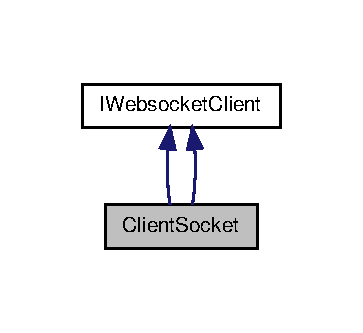
\includegraphics[width=174pt]{class_client_socket__inherit__graph}
\end{center}
\end{figure}


Collaboration diagram for Client\-Socket\-:
\nopagebreak
\begin{figure}[H]
\begin{center}
\leavevmode
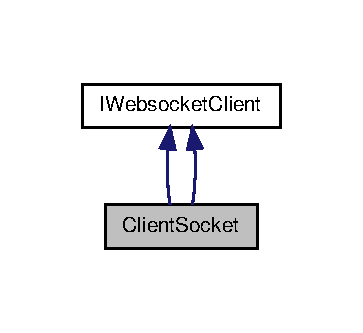
\includegraphics[width=174pt]{class_client_socket__coll__graph}
\end{center}
\end{figure}
\subsection*{Public Member Functions}
\begin{DoxyCompactItemize}
\item 
\hypertarget{class_client_socket_aa452c26d330984ce23eb98fba8e59c6a}{\hyperlink{class_client_socket_aa452c26d330984ce23eb98fba8e59c6a}{Client\-Socket} ()}\label{class_client_socket_aa452c26d330984ce23eb98fba8e59c6a}

\begin{DoxyCompactList}\small\item\em Client\-Socket\-Obj\-::\-Client\-Socket\-Obj Build one client. \end{DoxyCompactList}\item 
\hypertarget{class_client_socket_aef5d9c1c9b443124b820521276b175ca}{\hyperlink{class_client_socket_aef5d9c1c9b443124b820521276b175ca}{$\sim$\-Client\-Socket} ()}\label{class_client_socket_aef5d9c1c9b443124b820521276b175ca}

\begin{DoxyCompactList}\small\item\em \hyperlink{class_client_socket_aef5d9c1c9b443124b820521276b175ca}{Client\-Socket\-::$\sim$\-Client\-Socket} clean pointers. \end{DoxyCompactList}\item 
Q\-List$<$ std\-::string $>$ \hyperlink{class_client_socket_a1946057d900be8de8c6f66cedf0a607a}{websocket\-Parse} (Q\-Tcp\-Socket $\ast$socket)
\begin{DoxyCompactList}\small\item\em Client\-Socket\-Obj\-::websocket\-Parse decode websocket data from socket. \end{DoxyCompactList}\item 
void \hyperlink{class_client_socket_a5ec144ce9f5b71f11d861a5f94273bf2}{set\-Open} (bool open)
\begin{DoxyCompactList}\small\item\em Client\-Socket\-Obj\-::set\-Open set opening state for websocket. \end{DoxyCompactList}\item 
bool \hyperlink{class_client_socket_ab3747426831f271a9a0e54c5b44bddc7}{is\-Open} ()
\begin{DoxyCompactList}\small\item\em Client\-Socket\-Obj\-::is\-Open determine if websocket connection is O\-N. \end{DoxyCompactList}\item 
void \hyperlink{class_client_socket_a985fe4b2ab2ae12e4dbbd165580698ac}{set\-Websocket\-State} (bool state)
\begin{DoxyCompactList}\small\item\em Client\-Socket\-Obj\-::set\-Websocket\-State set E\-N\-A\-B\-L\-I\-N\-G state of websocket =$>$ mean socket connection will be maintained from that moment if state==true. \end{DoxyCompactList}\item 
bool \hyperlink{class_client_socket_a3ddc70db4798e5c8455a0ceecb470c70}{is\-Websocket\-Data} ()
\begin{DoxyCompactList}\small\item\em Client\-Socket\-Obj\-::is\-Websocket\-Data retrieve websocket E\-N\-A\-B\-L\-I\-N\-G state. \end{DoxyCompactList}\item 
int \hyperlink{class_client_socket_aedce28b93f08367feb6c43b808bb63e5}{close} ()
\item 
int \hyperlink{class_client_socket_ae2e6b6a4536c986b54d5db1902e11ce8}{send\-Message} (std\-::string message)
\item 
void \hyperlink{class_client_socket_af914375c58704f66d2819cac3a3cca67}{set\-Socket\-Client} (Q\-Tcp\-Socket $\ast$client\-Socket)
\begin{DoxyCompactList}\small\item\em set\-Socket\-Client Define client socket for this object \end{DoxyCompactList}\item 
\hypertarget{class_client_socket_aa452c26d330984ce23eb98fba8e59c6a}{\hyperlink{class_client_socket_aa452c26d330984ce23eb98fba8e59c6a}{Client\-Socket} ()}\label{class_client_socket_aa452c26d330984ce23eb98fba8e59c6a}

\begin{DoxyCompactList}\small\item\em Client\-Socket\-Obj\-::\-Client\-Socket\-Obj Build one client. \end{DoxyCompactList}\item 
Q\-List$<$ std\-::string $>$ \hyperlink{class_client_socket_aa9125ab7983520d0e536afef1be62c83}{websocket\-Parse} (Q\-Tcp\-Socket $\ast$socket)
\begin{DoxyCompactList}\small\item\em Client\-Socket\-Obj\-::websocket\-Parse decode websocket data from socket. \end{DoxyCompactList}\item 
void \hyperlink{class_client_socket_a5ec144ce9f5b71f11d861a5f94273bf2}{set\-Open} (bool open)
\begin{DoxyCompactList}\small\item\em Client\-Socket\-Obj\-::set\-Open set opening state for websocket. \end{DoxyCompactList}\item 
bool \hyperlink{class_client_socket_ab3747426831f271a9a0e54c5b44bddc7}{is\-Open} ()
\begin{DoxyCompactList}\small\item\em Client\-Socket\-Obj\-::is\-Open determine if websocket connection is O\-N. \end{DoxyCompactList}\item 
void \hyperlink{class_client_socket_a985fe4b2ab2ae12e4dbbd165580698ac}{set\-Websocket\-State} (bool state)
\begin{DoxyCompactList}\small\item\em Client\-Socket\-Obj\-::set\-Websocket\-State set E\-N\-A\-B\-L\-I\-N\-G state of websocket =$>$ mean socket connection will be maintained from that moment if state==true. \end{DoxyCompactList}\item 
bool \hyperlink{class_client_socket_a3ddc70db4798e5c8455a0ceecb470c70}{is\-Websocket\-Data} ()
\begin{DoxyCompactList}\small\item\em Client\-Socket\-Obj\-::is\-Websocket\-Data retrieve websocket E\-N\-A\-B\-L\-I\-N\-G state. \end{DoxyCompactList}\item 
int \hyperlink{class_client_socket_aedce28b93f08367feb6c43b808bb63e5}{close} ()
\item 
int \hyperlink{class_client_socket_ae2e6b6a4536c986b54d5db1902e11ce8}{send\-Message} (std\-::string message)
\item 
void \hyperlink{class_client_socket_af914375c58704f66d2819cac3a3cca67}{set\-Socket\-Client} (Q\-Tcp\-Socket $\ast$client\-Socket)
\begin{DoxyCompactList}\small\item\em set\-Socket\-Client Define client socket for this object \end{DoxyCompactList}\end{DoxyCompactItemize}


\subsection{Detailed Description}
clientsocket.\-h

websocket client object featuring one physical websocket connection

\begin{DoxyAuthor}{Author}
Bertrand Martel 
\end{DoxyAuthor}
\begin{DoxyVersion}{Version}
1.\-0 
\end{DoxyVersion}


\subsection{Member Function Documentation}
\hypertarget{class_client_socket_aedce28b93f08367feb6c43b808bb63e5}{\index{Client\-Socket@{Client\-Socket}!close@{close}}
\index{close@{close}!ClientSocket@{Client\-Socket}}
\subsubsection[{close}]{\setlength{\rightskip}{0pt plus 5cm}int Client\-Socket\-::close (
\begin{DoxyParamCaption}
{}
\end{DoxyParamCaption}
)\hspace{0.3cm}{\ttfamily [virtual]}}}\label{class_client_socket_aedce28b93f08367feb6c43b808bb63e5}
close websoclet client object

\begin{DoxyReturn}{Returns}
0 if success -\/1 if error 
\end{DoxyReturn}


Implements \hyperlink{class_i_websocket_client_ad20fddcd08c7880146fcd4ac20bb7b83}{I\-Websocket\-Client}.

\hypertarget{class_client_socket_aedce28b93f08367feb6c43b808bb63e5}{\index{Client\-Socket@{Client\-Socket}!close@{close}}
\index{close@{close}!ClientSocket@{Client\-Socket}}
\subsubsection[{close}]{\setlength{\rightskip}{0pt plus 5cm}int Client\-Socket\-::close (
\begin{DoxyParamCaption}
{}
\end{DoxyParamCaption}
)\hspace{0.3cm}{\ttfamily [virtual]}}}\label{class_client_socket_aedce28b93f08367feb6c43b808bb63e5}
close websoclet client object

\begin{DoxyReturn}{Returns}
0 if success -\/1 if error 
\end{DoxyReturn}


Implements \hyperlink{class_i_websocket_client_ad20fddcd08c7880146fcd4ac20bb7b83}{I\-Websocket\-Client}.

\hypertarget{class_client_socket_ab3747426831f271a9a0e54c5b44bddc7}{\index{Client\-Socket@{Client\-Socket}!is\-Open@{is\-Open}}
\index{is\-Open@{is\-Open}!ClientSocket@{Client\-Socket}}
\subsubsection[{is\-Open}]{\setlength{\rightskip}{0pt plus 5cm}bool Client\-Socket\-::is\-Open (
\begin{DoxyParamCaption}
{}
\end{DoxyParamCaption}
)}}\label{class_client_socket_ab3747426831f271a9a0e54c5b44bddc7}


Client\-Socket\-Obj\-::is\-Open determine if websocket connection is O\-N. 

\begin{DoxyReturn}{Returns}

\end{DoxyReturn}
\hypertarget{class_client_socket_ab3747426831f271a9a0e54c5b44bddc7}{\index{Client\-Socket@{Client\-Socket}!is\-Open@{is\-Open}}
\index{is\-Open@{is\-Open}!ClientSocket@{Client\-Socket}}
\subsubsection[{is\-Open}]{\setlength{\rightskip}{0pt plus 5cm}bool Client\-Socket\-::is\-Open (
\begin{DoxyParamCaption}
{}
\end{DoxyParamCaption}
)}}\label{class_client_socket_ab3747426831f271a9a0e54c5b44bddc7}


Client\-Socket\-Obj\-::is\-Open determine if websocket connection is O\-N. 

\begin{DoxyReturn}{Returns}

\end{DoxyReturn}
\hypertarget{class_client_socket_a3ddc70db4798e5c8455a0ceecb470c70}{\index{Client\-Socket@{Client\-Socket}!is\-Websocket\-Data@{is\-Websocket\-Data}}
\index{is\-Websocket\-Data@{is\-Websocket\-Data}!ClientSocket@{Client\-Socket}}
\subsubsection[{is\-Websocket\-Data}]{\setlength{\rightskip}{0pt plus 5cm}bool Client\-Socket\-::is\-Websocket\-Data (
\begin{DoxyParamCaption}
{}
\end{DoxyParamCaption}
)}}\label{class_client_socket_a3ddc70db4798e5c8455a0ceecb470c70}


Client\-Socket\-Obj\-::is\-Websocket\-Data retrieve websocket E\-N\-A\-B\-L\-I\-N\-G state. 

\begin{DoxyReturn}{Returns}
state 
\end{DoxyReturn}
\hypertarget{class_client_socket_a3ddc70db4798e5c8455a0ceecb470c70}{\index{Client\-Socket@{Client\-Socket}!is\-Websocket\-Data@{is\-Websocket\-Data}}
\index{is\-Websocket\-Data@{is\-Websocket\-Data}!ClientSocket@{Client\-Socket}}
\subsubsection[{is\-Websocket\-Data}]{\setlength{\rightskip}{0pt plus 5cm}bool Client\-Socket\-::is\-Websocket\-Data (
\begin{DoxyParamCaption}
{}
\end{DoxyParamCaption}
)}}\label{class_client_socket_a3ddc70db4798e5c8455a0ceecb470c70}


Client\-Socket\-Obj\-::is\-Websocket\-Data retrieve websocket E\-N\-A\-B\-L\-I\-N\-G state. 

\begin{DoxyReturn}{Returns}
state 
\end{DoxyReturn}
\hypertarget{class_client_socket_ae2e6b6a4536c986b54d5db1902e11ce8}{\index{Client\-Socket@{Client\-Socket}!send\-Message@{send\-Message}}
\index{send\-Message@{send\-Message}!ClientSocket@{Client\-Socket}}
\subsubsection[{send\-Message}]{\setlength{\rightskip}{0pt plus 5cm}int Client\-Socket\-::send\-Message (
\begin{DoxyParamCaption}
\item[{std\-::string}]{message}
\end{DoxyParamCaption}
)\hspace{0.3cm}{\ttfamily [virtual]}}}\label{class_client_socket_ae2e6b6a4536c986b54d5db1902e11ce8}
Send a message to websocket client


\begin{DoxyParams}{Parameters}
{\em string} & Message to be sent to client \\
\hline
\end{DoxyParams}
\begin{DoxyReturn}{Returns}
0 if success -\/1 if error 
\end{DoxyReturn}


Implements \hyperlink{class_i_websocket_client_ac2178027869dc142fe924858d59fc9c1}{I\-Websocket\-Client}.

\hypertarget{class_client_socket_ae2e6b6a4536c986b54d5db1902e11ce8}{\index{Client\-Socket@{Client\-Socket}!send\-Message@{send\-Message}}
\index{send\-Message@{send\-Message}!ClientSocket@{Client\-Socket}}
\subsubsection[{send\-Message}]{\setlength{\rightskip}{0pt plus 5cm}int Client\-Socket\-::send\-Message (
\begin{DoxyParamCaption}
\item[{std\-::string}]{message}
\end{DoxyParamCaption}
)\hspace{0.3cm}{\ttfamily [virtual]}}}\label{class_client_socket_ae2e6b6a4536c986b54d5db1902e11ce8}
Send a message to websocket client


\begin{DoxyParams}{Parameters}
{\em string} & Message to be sent to client \\
\hline
\end{DoxyParams}
\begin{DoxyReturn}{Returns}
0 if success -\/1 if error 
\end{DoxyReturn}


Implements \hyperlink{class_i_websocket_client_ac2178027869dc142fe924858d59fc9c1}{I\-Websocket\-Client}.

\hypertarget{class_client_socket_a5ec144ce9f5b71f11d861a5f94273bf2}{\index{Client\-Socket@{Client\-Socket}!set\-Open@{set\-Open}}
\index{set\-Open@{set\-Open}!ClientSocket@{Client\-Socket}}
\subsubsection[{set\-Open}]{\setlength{\rightskip}{0pt plus 5cm}void Client\-Socket\-::set\-Open (
\begin{DoxyParamCaption}
\item[{bool}]{open}
\end{DoxyParamCaption}
)}}\label{class_client_socket_a5ec144ce9f5b71f11d861a5f94273bf2}


Client\-Socket\-Obj\-::set\-Open set opening state for websocket. 


\begin{DoxyParams}{Parameters}
{\em open} & opening state \\
\hline
\end{DoxyParams}
\hypertarget{class_client_socket_a5ec144ce9f5b71f11d861a5f94273bf2}{\index{Client\-Socket@{Client\-Socket}!set\-Open@{set\-Open}}
\index{set\-Open@{set\-Open}!ClientSocket@{Client\-Socket}}
\subsubsection[{set\-Open}]{\setlength{\rightskip}{0pt plus 5cm}void Client\-Socket\-::set\-Open (
\begin{DoxyParamCaption}
\item[{bool}]{open}
\end{DoxyParamCaption}
)}}\label{class_client_socket_a5ec144ce9f5b71f11d861a5f94273bf2}


Client\-Socket\-Obj\-::set\-Open set opening state for websocket. 


\begin{DoxyParams}{Parameters}
{\em open} & opening state \\
\hline
\end{DoxyParams}
\hypertarget{class_client_socket_af914375c58704f66d2819cac3a3cca67}{\index{Client\-Socket@{Client\-Socket}!set\-Socket\-Client@{set\-Socket\-Client}}
\index{set\-Socket\-Client@{set\-Socket\-Client}!ClientSocket@{Client\-Socket}}
\subsubsection[{set\-Socket\-Client}]{\setlength{\rightskip}{0pt plus 5cm}void Client\-Socket\-::set\-Socket\-Client (
\begin{DoxyParamCaption}
\item[{Q\-Tcp\-Socket $\ast$}]{client\-Socket}
\end{DoxyParamCaption}
)}}\label{class_client_socket_af914375c58704f66d2819cac3a3cca67}


set\-Socket\-Client Define client socket for this object 


\begin{DoxyParams}{Parameters}
{\em client\-Socket} & client socket \\
\hline
\end{DoxyParams}
\hypertarget{class_client_socket_af914375c58704f66d2819cac3a3cca67}{\index{Client\-Socket@{Client\-Socket}!set\-Socket\-Client@{set\-Socket\-Client}}
\index{set\-Socket\-Client@{set\-Socket\-Client}!ClientSocket@{Client\-Socket}}
\subsubsection[{set\-Socket\-Client}]{\setlength{\rightskip}{0pt plus 5cm}void Client\-Socket\-::set\-Socket\-Client (
\begin{DoxyParamCaption}
\item[{Q\-Tcp\-Socket $\ast$}]{client\-Socket}
\end{DoxyParamCaption}
)}}\label{class_client_socket_af914375c58704f66d2819cac3a3cca67}


set\-Socket\-Client Define client socket for this object 

set\-Socket\-Client set socket client socket


\begin{DoxyParams}{Parameters}
{\em client\-Socket} & client socket\\
\hline
{\em client\-Socket} & \\
\hline
\end{DoxyParams}
\hypertarget{class_client_socket_a985fe4b2ab2ae12e4dbbd165580698ac}{\index{Client\-Socket@{Client\-Socket}!set\-Websocket\-State@{set\-Websocket\-State}}
\index{set\-Websocket\-State@{set\-Websocket\-State}!ClientSocket@{Client\-Socket}}
\subsubsection[{set\-Websocket\-State}]{\setlength{\rightskip}{0pt plus 5cm}void Client\-Socket\-::set\-Websocket\-State (
\begin{DoxyParamCaption}
\item[{bool}]{state}
\end{DoxyParamCaption}
)}}\label{class_client_socket_a985fe4b2ab2ae12e4dbbd165580698ac}


Client\-Socket\-Obj\-::set\-Websocket\-State set E\-N\-A\-B\-L\-I\-N\-G state of websocket =$>$ mean socket connection will be maintained from that moment if state==true. 


\begin{DoxyParams}{Parameters}
{\em state} & \\
\hline
\end{DoxyParams}
\hypertarget{class_client_socket_a985fe4b2ab2ae12e4dbbd165580698ac}{\index{Client\-Socket@{Client\-Socket}!set\-Websocket\-State@{set\-Websocket\-State}}
\index{set\-Websocket\-State@{set\-Websocket\-State}!ClientSocket@{Client\-Socket}}
\subsubsection[{set\-Websocket\-State}]{\setlength{\rightskip}{0pt plus 5cm}void Client\-Socket\-::set\-Websocket\-State (
\begin{DoxyParamCaption}
\item[{bool}]{state}
\end{DoxyParamCaption}
)}}\label{class_client_socket_a985fe4b2ab2ae12e4dbbd165580698ac}


Client\-Socket\-Obj\-::set\-Websocket\-State set E\-N\-A\-B\-L\-I\-N\-G state of websocket =$>$ mean socket connection will be maintained from that moment if state==true. 


\begin{DoxyParams}{Parameters}
{\em state} & \\
\hline
\end{DoxyParams}
\hypertarget{class_client_socket_aa9125ab7983520d0e536afef1be62c83}{\index{Client\-Socket@{Client\-Socket}!websocket\-Parse@{websocket\-Parse}}
\index{websocket\-Parse@{websocket\-Parse}!ClientSocket@{Client\-Socket}}
\subsubsection[{websocket\-Parse}]{\setlength{\rightskip}{0pt plus 5cm}Q\-List$<$std\-::string$>$ Client\-Socket\-::websocket\-Parse (
\begin{DoxyParamCaption}
\item[{Q\-Tcp\-Socket $\ast$}]{socket}
\end{DoxyParamCaption}
)}}\label{class_client_socket_aa9125ab7983520d0e536afef1be62c83}


Client\-Socket\-Obj\-::websocket\-Parse decode websocket data from socket. 


\begin{DoxyParams}{Parameters}
{\em socket} & client socket \\
\hline
\end{DoxyParams}
\begin{DoxyReturn}{Returns}
list of string message decoded from websocket 
\end{DoxyReturn}
\hypertarget{class_client_socket_a1946057d900be8de8c6f66cedf0a607a}{\index{Client\-Socket@{Client\-Socket}!websocket\-Parse@{websocket\-Parse}}
\index{websocket\-Parse@{websocket\-Parse}!ClientSocket@{Client\-Socket}}
\subsubsection[{websocket\-Parse}]{\setlength{\rightskip}{0pt plus 5cm}Q\-List$<$ string $>$ Client\-Socket\-::websocket\-Parse (
\begin{DoxyParamCaption}
\item[{Q\-Tcp\-Socket $\ast$}]{socket}
\end{DoxyParamCaption}
)}}\label{class_client_socket_a1946057d900be8de8c6f66cedf0a607a}


Client\-Socket\-Obj\-::websocket\-Parse decode websocket data from socket. 


\begin{DoxyParams}{Parameters}
{\em socket} & client socket \\
\hline
\end{DoxyParams}
\begin{DoxyReturn}{Returns}
list of string message decoded from websocket 
\end{DoxyReturn}


The documentation for this class was generated from the following files\-:\begin{DoxyCompactItemize}
\item 
/home/abathur/\-Bureau/open\-\_\-source/websocketcpp/libwebsocket/protocol/websocket/client\-Socket.\-h\item 
/home/abathur/\-Bureau/open\-\_\-source/websocketcpp/libwebsocket/release/protocol/websocket/client\-Socket.\-h\item 
/home/abathur/\-Bureau/open\-\_\-source/websocketcpp/libwebsocket/protocol/websocket/client\-Socket.\-cpp\end{DoxyCompactItemize}

\hypertarget{class_i_client_event_listener}{\section{I\-Client\-Event\-Listener Class Reference}
\label{class_i_client_event_listener}\index{I\-Client\-Event\-Listener@{I\-Client\-Event\-Listener}}
}


The \hyperlink{class_i_client_event_listener}{I\-Client\-Event\-Listener} class Client Socket event listener template class.  




{\ttfamily \#include $<$I\-Client\-Event\-Listener.\-h$>$}

\subsection*{Public Member Functions}
\begin{DoxyCompactItemize}
\item 
virtual void \hyperlink{class_i_client_event_listener_ad361206cbbc2f53df38d41b00c088734}{on\-Client\-Close} (\hyperlink{class_i_websocket_client}{I\-Websocket\-Client} \&client)=0
\item 
virtual void \hyperlink{class_i_client_event_listener_ab224b5ffe68d956417da32661feb9f93}{on\-Client\-Connection} (\hyperlink{class_i_websocket_client}{I\-Websocket\-Client} \&client)=0
\item 
virtual void \hyperlink{class_i_client_event_listener_a69cdb3e0149213614301de11305e71a1}{on\-Message\-Received\-From\-Client} (\hyperlink{class_i_websocket_client}{I\-Websocket\-Client} \&client, std\-::string message)=0
\item 
virtual void \hyperlink{class_i_client_event_listener_ad361206cbbc2f53df38d41b00c088734}{on\-Client\-Close} (\hyperlink{class_i_websocket_client}{I\-Websocket\-Client} \&client)=0
\item 
virtual void \hyperlink{class_i_client_event_listener_ab224b5ffe68d956417da32661feb9f93}{on\-Client\-Connection} (\hyperlink{class_i_websocket_client}{I\-Websocket\-Client} \&client)=0
\item 
virtual void \hyperlink{class_i_client_event_listener_a69cdb3e0149213614301de11305e71a1}{on\-Message\-Received\-From\-Client} (\hyperlink{class_i_websocket_client}{I\-Websocket\-Client} \&client, std\-::string message)=0
\end{DoxyCompactItemize}


\subsection{Detailed Description}
The \hyperlink{class_i_client_event_listener}{I\-Client\-Event\-Listener} class Client Socket event listener template class. 

I\-Client\-Event\-Listener.\-h

Define all client socket event that can happen and that will pop event in class that will inherit this one

\begin{DoxyAuthor}{Author}
Bertrand Martel 
\end{DoxyAuthor}
\begin{DoxyVersion}{Version}
1.\-0 
\end{DoxyVersion}


\subsection{Member Function Documentation}
\hypertarget{class_i_client_event_listener_ad361206cbbc2f53df38d41b00c088734}{\index{I\-Client\-Event\-Listener@{I\-Client\-Event\-Listener}!on\-Client\-Close@{on\-Client\-Close}}
\index{on\-Client\-Close@{on\-Client\-Close}!IClientEventListener@{I\-Client\-Event\-Listener}}
\subsubsection[{on\-Client\-Close}]{\setlength{\rightskip}{0pt plus 5cm}virtual void I\-Client\-Event\-Listener\-::on\-Client\-Close (
\begin{DoxyParamCaption}
\item[{{\bf I\-Websocket\-Client} \&}]{client}
\end{DoxyParamCaption}
)\hspace{0.3cm}{\ttfamily [pure virtual]}}}\label{class_i_client_event_listener_ad361206cbbc2f53df38d41b00c088734}
called when a websocket client connection closes


\begin{DoxyParams}{Parameters}
{\em client\-Ref} & \\
\hline
\end{DoxyParams}
\hypertarget{class_i_client_event_listener_ad361206cbbc2f53df38d41b00c088734}{\index{I\-Client\-Event\-Listener@{I\-Client\-Event\-Listener}!on\-Client\-Close@{on\-Client\-Close}}
\index{on\-Client\-Close@{on\-Client\-Close}!IClientEventListener@{I\-Client\-Event\-Listener}}
\subsubsection[{on\-Client\-Close}]{\setlength{\rightskip}{0pt plus 5cm}virtual void I\-Client\-Event\-Listener\-::on\-Client\-Close (
\begin{DoxyParamCaption}
\item[{{\bf I\-Websocket\-Client} \&}]{client}
\end{DoxyParamCaption}
)\hspace{0.3cm}{\ttfamily [pure virtual]}}}\label{class_i_client_event_listener_ad361206cbbc2f53df38d41b00c088734}
called when a websocket client connection closes


\begin{DoxyParams}{Parameters}
{\em client\-Ref} & \\
\hline
\end{DoxyParams}
\hypertarget{class_i_client_event_listener_ab224b5ffe68d956417da32661feb9f93}{\index{I\-Client\-Event\-Listener@{I\-Client\-Event\-Listener}!on\-Client\-Connection@{on\-Client\-Connection}}
\index{on\-Client\-Connection@{on\-Client\-Connection}!IClientEventListener@{I\-Client\-Event\-Listener}}
\subsubsection[{on\-Client\-Connection}]{\setlength{\rightskip}{0pt plus 5cm}virtual void I\-Client\-Event\-Listener\-::on\-Client\-Connection (
\begin{DoxyParamCaption}
\item[{{\bf I\-Websocket\-Client} \&}]{client}
\end{DoxyParamCaption}
)\hspace{0.3cm}{\ttfamily [pure virtual]}}}\label{class_i_client_event_listener_ab224b5ffe68d956417da32661feb9f93}
called when a websocket client has successfully connected to server


\begin{DoxyParams}{Parameters}
{\em client} & \\
\hline
\end{DoxyParams}
\hypertarget{class_i_client_event_listener_ab224b5ffe68d956417da32661feb9f93}{\index{I\-Client\-Event\-Listener@{I\-Client\-Event\-Listener}!on\-Client\-Connection@{on\-Client\-Connection}}
\index{on\-Client\-Connection@{on\-Client\-Connection}!IClientEventListener@{I\-Client\-Event\-Listener}}
\subsubsection[{on\-Client\-Connection}]{\setlength{\rightskip}{0pt plus 5cm}virtual void I\-Client\-Event\-Listener\-::on\-Client\-Connection (
\begin{DoxyParamCaption}
\item[{{\bf I\-Websocket\-Client} \&}]{client}
\end{DoxyParamCaption}
)\hspace{0.3cm}{\ttfamily [pure virtual]}}}\label{class_i_client_event_listener_ab224b5ffe68d956417da32661feb9f93}
called when a websocket client has successfully connected to server


\begin{DoxyParams}{Parameters}
{\em client} & \\
\hline
\end{DoxyParams}
\hypertarget{class_i_client_event_listener_a69cdb3e0149213614301de11305e71a1}{\index{I\-Client\-Event\-Listener@{I\-Client\-Event\-Listener}!on\-Message\-Received\-From\-Client@{on\-Message\-Received\-From\-Client}}
\index{on\-Message\-Received\-From\-Client@{on\-Message\-Received\-From\-Client}!IClientEventListener@{I\-Client\-Event\-Listener}}
\subsubsection[{on\-Message\-Received\-From\-Client}]{\setlength{\rightskip}{0pt plus 5cm}virtual void I\-Client\-Event\-Listener\-::on\-Message\-Received\-From\-Client (
\begin{DoxyParamCaption}
\item[{{\bf I\-Websocket\-Client} \&}]{client, }
\item[{std\-::string}]{message}
\end{DoxyParamCaption}
)\hspace{0.3cm}{\ttfamily [pure virtual]}}}\label{class_i_client_event_listener_a69cdb3e0149213614301de11305e71a1}
called when a message has been received from client


\begin{DoxyParams}{Parameters}
{\em client} & client object \\
\hline
{\em message} & message delivered \\
\hline
\end{DoxyParams}
\hypertarget{class_i_client_event_listener_a69cdb3e0149213614301de11305e71a1}{\index{I\-Client\-Event\-Listener@{I\-Client\-Event\-Listener}!on\-Message\-Received\-From\-Client@{on\-Message\-Received\-From\-Client}}
\index{on\-Message\-Received\-From\-Client@{on\-Message\-Received\-From\-Client}!IClientEventListener@{I\-Client\-Event\-Listener}}
\subsubsection[{on\-Message\-Received\-From\-Client}]{\setlength{\rightskip}{0pt plus 5cm}virtual void I\-Client\-Event\-Listener\-::on\-Message\-Received\-From\-Client (
\begin{DoxyParamCaption}
\item[{{\bf I\-Websocket\-Client} \&}]{client, }
\item[{std\-::string}]{message}
\end{DoxyParamCaption}
)\hspace{0.3cm}{\ttfamily [pure virtual]}}}\label{class_i_client_event_listener_a69cdb3e0149213614301de11305e71a1}
called when a message has been received from client


\begin{DoxyParams}{Parameters}
{\em client} & client object \\
\hline
{\em message} & message delivered \\
\hline
\end{DoxyParams}


The documentation for this class was generated from the following files\-:\begin{DoxyCompactItemize}
\item 
/home/abathur/\-Bureau/open\-\_\-source/websocketcpp/libwebsocket/protocol/websocket/I\-Client\-Event\-Listener.\-h\item 
/home/abathur/\-Bureau/open\-\_\-source/websocketcpp/libwebsocket/release/protocol/websocket/I\-Client\-Event\-Listener.\-h\end{DoxyCompactItemize}

\hypertarget{class_i_websocket_client}{\section{I\-Websocket\-Client Class Reference}
\label{class_i_websocket_client}\index{I\-Websocket\-Client@{I\-Websocket\-Client}}
}


{\ttfamily \#include $<$I\-Websocket\-Client.\-h$>$}



Inheritance diagram for I\-Websocket\-Client\-:
\nopagebreak
\begin{figure}[H]
\begin{center}
\leavevmode
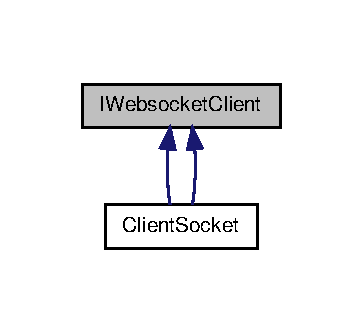
\includegraphics[width=174pt]{class_i_websocket_client__inherit__graph}
\end{center}
\end{figure}
\subsection*{Public Member Functions}
\begin{DoxyCompactItemize}
\item 
virtual int \hyperlink{class_i_websocket_client_ad20fddcd08c7880146fcd4ac20bb7b83}{close} ()=0
\item 
virtual int \hyperlink{class_i_websocket_client_ac2178027869dc142fe924858d59fc9c1}{send\-Message} (std\-::string message)=0
\item 
virtual int \hyperlink{class_i_websocket_client_ad20fddcd08c7880146fcd4ac20bb7b83}{close} ()=0
\item 
virtual int \hyperlink{class_i_websocket_client_ac2178027869dc142fe924858d59fc9c1}{send\-Message} (std\-::string message)=0
\end{DoxyCompactItemize}


\subsection{Detailed Description}
I\-Websocket\-Client.\-h

Define generic template for websocket client socket

\begin{DoxyAuthor}{Author}
Bertrand Martel 
\end{DoxyAuthor}
\begin{DoxyVersion}{Version}
1.\-0 
\end{DoxyVersion}


\subsection{Member Function Documentation}
\hypertarget{class_i_websocket_client_ad20fddcd08c7880146fcd4ac20bb7b83}{\index{I\-Websocket\-Client@{I\-Websocket\-Client}!close@{close}}
\index{close@{close}!IWebsocketClient@{I\-Websocket\-Client}}
\subsubsection[{close}]{\setlength{\rightskip}{0pt plus 5cm}virtual int I\-Websocket\-Client\-::close (
\begin{DoxyParamCaption}
{}
\end{DoxyParamCaption}
)\hspace{0.3cm}{\ttfamily [pure virtual]}}}\label{class_i_websocket_client_ad20fddcd08c7880146fcd4ac20bb7b83}
close websoclet client object

\begin{DoxyReturn}{Returns}
0 if success -\/1 if error 
\end{DoxyReturn}


Implemented in \hyperlink{class_client_socket_aedce28b93f08367feb6c43b808bb63e5}{Client\-Socket}, and \hyperlink{class_client_socket_aedce28b93f08367feb6c43b808bb63e5}{Client\-Socket}.

\hypertarget{class_i_websocket_client_ad20fddcd08c7880146fcd4ac20bb7b83}{\index{I\-Websocket\-Client@{I\-Websocket\-Client}!close@{close}}
\index{close@{close}!IWebsocketClient@{I\-Websocket\-Client}}
\subsubsection[{close}]{\setlength{\rightskip}{0pt plus 5cm}virtual int I\-Websocket\-Client\-::close (
\begin{DoxyParamCaption}
{}
\end{DoxyParamCaption}
)\hspace{0.3cm}{\ttfamily [pure virtual]}}}\label{class_i_websocket_client_ad20fddcd08c7880146fcd4ac20bb7b83}
close websoclet client object

\begin{DoxyReturn}{Returns}
0 if success -\/1 if error 
\end{DoxyReturn}


Implemented in \hyperlink{class_client_socket_aedce28b93f08367feb6c43b808bb63e5}{Client\-Socket}, and \hyperlink{class_client_socket_aedce28b93f08367feb6c43b808bb63e5}{Client\-Socket}.

\hypertarget{class_i_websocket_client_ac2178027869dc142fe924858d59fc9c1}{\index{I\-Websocket\-Client@{I\-Websocket\-Client}!send\-Message@{send\-Message}}
\index{send\-Message@{send\-Message}!IWebsocketClient@{I\-Websocket\-Client}}
\subsubsection[{send\-Message}]{\setlength{\rightskip}{0pt plus 5cm}virtual int I\-Websocket\-Client\-::send\-Message (
\begin{DoxyParamCaption}
\item[{std\-::string}]{message}
\end{DoxyParamCaption}
)\hspace{0.3cm}{\ttfamily [pure virtual]}}}\label{class_i_websocket_client_ac2178027869dc142fe924858d59fc9c1}
Send a message to websocket client


\begin{DoxyParams}{Parameters}
{\em string} & Message to be sent to client \\
\hline
\end{DoxyParams}
\begin{DoxyReturn}{Returns}
0 if success -\/1 if error 
\end{DoxyReturn}


Implemented in \hyperlink{class_client_socket_ae2e6b6a4536c986b54d5db1902e11ce8}{Client\-Socket}, and \hyperlink{class_client_socket_ae2e6b6a4536c986b54d5db1902e11ce8}{Client\-Socket}.

\hypertarget{class_i_websocket_client_ac2178027869dc142fe924858d59fc9c1}{\index{I\-Websocket\-Client@{I\-Websocket\-Client}!send\-Message@{send\-Message}}
\index{send\-Message@{send\-Message}!IWebsocketClient@{I\-Websocket\-Client}}
\subsubsection[{send\-Message}]{\setlength{\rightskip}{0pt plus 5cm}virtual int I\-Websocket\-Client\-::send\-Message (
\begin{DoxyParamCaption}
\item[{std\-::string}]{message}
\end{DoxyParamCaption}
)\hspace{0.3cm}{\ttfamily [pure virtual]}}}\label{class_i_websocket_client_ac2178027869dc142fe924858d59fc9c1}
Send a message to websocket client


\begin{DoxyParams}{Parameters}
{\em string} & Message to be sent to client \\
\hline
\end{DoxyParams}
\begin{DoxyReturn}{Returns}
0 if success -\/1 if error 
\end{DoxyReturn}


Implemented in \hyperlink{class_client_socket_ae2e6b6a4536c986b54d5db1902e11ce8}{Client\-Socket}, and \hyperlink{class_client_socket_ae2e6b6a4536c986b54d5db1902e11ce8}{Client\-Socket}.



The documentation for this class was generated from the following files\-:\begin{DoxyCompactItemize}
\item 
/home/abathur/\-Bureau/open\-\_\-source/websocketcpp/libwebsocket/protocol/websocket/I\-Websocket\-Client.\-h\item 
/home/abathur/\-Bureau/open\-\_\-source/websocketcpp/libwebsocket/release/protocol/websocket/I\-Websocket\-Client.\-h\end{DoxyCompactItemize}

\hypertarget{classstringutils}{\section{stringutils Class Reference}
\label{classstringutils}\index{stringutils@{stringutils}}
}


The stringutils class String utility functions.  




{\ttfamily \#include $<$stringutils.\-h$>$}

\subsection*{Static Public Member Functions}
\begin{DoxyCompactItemize}
\item 
static std\-::vector$<$ std\-::string $>$ \hyperlink{classstringutils_a20745a2b1f3ae2a4c863e65838fc1bef}{split} (const std\-::string \&s, char delim)
\begin{DoxyCompactList}\small\item\em split split a string with a character delimiter \end{DoxyCompactList}\item 
static std\-::vector$<$ std\-::string $>$ \hyperlink{classstringutils_a9d2982b0d17c5fe3911bf1b08ecef115}{split} (const std\-::string \&s, char delim, std\-::vector$<$ std\-::string $>$ \&elems)
\begin{DoxyCompactList}\small\item\em split split a string with a character delimiter \end{DoxyCompactList}\item 
static bool \hyperlink{classstringutils_a945219b9581cac4b3254deac35e9ab02}{is\-Num} (char $\ast$s)
\begin{DoxyCompactList}\small\item\em is\-Num check if char $\ast$ is numeric data \end{DoxyCompactList}\item 
\hypertarget{classstringutils_afb1addddb00afafa45447dc16e73a320}{static std\-::string \& {\bfseries ltrim} (std\-::string \&s)}\label{classstringutils_afb1addddb00afafa45447dc16e73a320}

\item 
\hypertarget{classstringutils_a7326b94129fb258d0ed42e0228b3a5b2}{static std\-::string \& {\bfseries rtrim} (std\-::string \&s)}\label{classstringutils_a7326b94129fb258d0ed42e0228b3a5b2}

\item 
\hypertarget{classstringutils_a1b03731449410613ccb73f0213036dac}{static std\-::string \& {\bfseries trim} (std\-::string \&s)}\label{classstringutils_a1b03731449410613ccb73f0213036dac}

\item 
static std\-::vector$<$ std\-::string $>$ \hyperlink{classstringutils_a20745a2b1f3ae2a4c863e65838fc1bef}{split} (const std\-::string \&s, char delim)
\begin{DoxyCompactList}\small\item\em split split a string with a character delimiter \end{DoxyCompactList}\item 
static std\-::vector$<$ std\-::string $>$ \hyperlink{classstringutils_a9d2982b0d17c5fe3911bf1b08ecef115}{split} (const std\-::string \&s, char delim, std\-::vector$<$ std\-::string $>$ \&elems)
\begin{DoxyCompactList}\small\item\em split split a string with a character delimiter \end{DoxyCompactList}\item 
static bool \hyperlink{classstringutils_a75dff8d4b767b34d3c25add0baea6ffc}{is\-Num} (char $\ast$s)
\begin{DoxyCompactList}\small\item\em is\-Num check if char $\ast$ is numeric data \end{DoxyCompactList}\item 
\hypertarget{classstringutils_afb1addddb00afafa45447dc16e73a320}{static std\-::string \& {\bfseries ltrim} (std\-::string \&s)}\label{classstringutils_afb1addddb00afafa45447dc16e73a320}

\item 
\hypertarget{classstringutils_a7326b94129fb258d0ed42e0228b3a5b2}{static std\-::string \& {\bfseries rtrim} (std\-::string \&s)}\label{classstringutils_a7326b94129fb258d0ed42e0228b3a5b2}

\item 
\hypertarget{classstringutils_a1b03731449410613ccb73f0213036dac}{static std\-::string \& {\bfseries trim} (std\-::string \&s)}\label{classstringutils_a1b03731449410613ccb73f0213036dac}

\end{DoxyCompactItemize}


\subsection{Detailed Description}
The stringutils class String utility functions. 

stringutils.\-h Utility funcions for http parser

\begin{DoxyAuthor}{Author}
Bertrand Martel 
\end{DoxyAuthor}
\begin{DoxyVersion}{Version}
1.\-0 
\end{DoxyVersion}


\subsection{Member Function Documentation}
\hypertarget{classstringutils_a945219b9581cac4b3254deac35e9ab02}{\index{stringutils@{stringutils}!is\-Num@{is\-Num}}
\index{is\-Num@{is\-Num}!stringutils@{stringutils}}
\subsubsection[{is\-Num}]{\setlength{\rightskip}{0pt plus 5cm}bool stringutils\-::is\-Num (
\begin{DoxyParamCaption}
\item[{char $\ast$}]{s}
\end{DoxyParamCaption}
)\hspace{0.3cm}{\ttfamily [static]}}}\label{classstringutils_a945219b9581cac4b3254deac35e9ab02}


is\-Num check if char $\ast$ is numeric data 


\begin{DoxyParams}{Parameters}
{\em s} & char $\ast$ input \\
\hline
\end{DoxyParams}
\begin{DoxyReturn}{Returns}
true if data is numeric 
\end{DoxyReturn}
\hypertarget{classstringutils_a75dff8d4b767b34d3c25add0baea6ffc}{\index{stringutils@{stringutils}!is\-Num@{is\-Num}}
\index{is\-Num@{is\-Num}!stringutils@{stringutils}}
\subsubsection[{is\-Num}]{\setlength{\rightskip}{0pt plus 5cm}static bool stringutils\-::is\-Num (
\begin{DoxyParamCaption}
\item[{char $\ast$}]{s}
\end{DoxyParamCaption}
)\hspace{0.3cm}{\ttfamily [static]}}}\label{classstringutils_a75dff8d4b767b34d3c25add0baea6ffc}


is\-Num check if char $\ast$ is numeric data 


\begin{DoxyParams}{Parameters}
{\em s} & char $\ast$ input \\
\hline
\end{DoxyParams}
\begin{DoxyReturn}{Returns}
true if data is numeric 
\end{DoxyReturn}
\hypertarget{classstringutils_a20745a2b1f3ae2a4c863e65838fc1bef}{\index{stringutils@{stringutils}!split@{split}}
\index{split@{split}!stringutils@{stringutils}}
\subsubsection[{split}]{\setlength{\rightskip}{0pt plus 5cm}static std\-::vector$<$std\-::string$>$ stringutils\-::split (
\begin{DoxyParamCaption}
\item[{const std\-::string \&}]{s, }
\item[{char}]{delim}
\end{DoxyParamCaption}
)\hspace{0.3cm}{\ttfamily [static]}}}\label{classstringutils_a20745a2b1f3ae2a4c863e65838fc1bef}


split split a string with a character delimiter 


\begin{DoxyParams}{Parameters}
{\em s} & string to split \\
\hline
{\em delim} & character delimiter \\
\hline
\end{DoxyParams}
\begin{DoxyReturn}{Returns}
vector of splitted string 
\end{DoxyReturn}
\hypertarget{classstringutils_a20745a2b1f3ae2a4c863e65838fc1bef}{\index{stringutils@{stringutils}!split@{split}}
\index{split@{split}!stringutils@{stringutils}}
\subsubsection[{split}]{\setlength{\rightskip}{0pt plus 5cm}static std\-::vector$<$std\-::string$>$ stringutils\-::split (
\begin{DoxyParamCaption}
\item[{const std\-::string \&}]{s, }
\item[{char}]{delim}
\end{DoxyParamCaption}
)\hspace{0.3cm}{\ttfamily [static]}}}\label{classstringutils_a20745a2b1f3ae2a4c863e65838fc1bef}


split split a string with a character delimiter 


\begin{DoxyParams}{Parameters}
{\em s} & string to split \\
\hline
{\em delim} & character delimiter \\
\hline
\end{DoxyParams}
\begin{DoxyReturn}{Returns}
vector of splitted string 
\end{DoxyReturn}
\hypertarget{classstringutils_a9d2982b0d17c5fe3911bf1b08ecef115}{\index{stringutils@{stringutils}!split@{split}}
\index{split@{split}!stringutils@{stringutils}}
\subsubsection[{split}]{\setlength{\rightskip}{0pt plus 5cm}static std\-::vector$<$std\-::string$>$ stringutils\-::split (
\begin{DoxyParamCaption}
\item[{const std\-::string \&}]{s, }
\item[{char}]{delim, }
\item[{std\-::vector$<$ std\-::string $>$ \&}]{elems}
\end{DoxyParamCaption}
)\hspace{0.3cm}{\ttfamily [static]}}}\label{classstringutils_a9d2982b0d17c5fe3911bf1b08ecef115}


split split a string with a character delimiter 


\begin{DoxyParams}{Parameters}
{\em s} & string to split \\
\hline
{\em delim} & character delimiter \\
\hline
{\em elems} & the same as vector list returned \\
\hline
\end{DoxyParams}
\begin{DoxyReturn}{Returns}
vector of splitted string 
\end{DoxyReturn}
\hypertarget{classstringutils_a9d2982b0d17c5fe3911bf1b08ecef115}{\index{stringutils@{stringutils}!split@{split}}
\index{split@{split}!stringutils@{stringutils}}
\subsubsection[{split}]{\setlength{\rightskip}{0pt plus 5cm}static std\-::vector$<$std\-::string$>$ stringutils\-::split (
\begin{DoxyParamCaption}
\item[{const std\-::string \&}]{s, }
\item[{char}]{delim, }
\item[{std\-::vector$<$ std\-::string $>$ \&}]{elems}
\end{DoxyParamCaption}
)\hspace{0.3cm}{\ttfamily [static]}}}\label{classstringutils_a9d2982b0d17c5fe3911bf1b08ecef115}


split split a string with a character delimiter 


\begin{DoxyParams}{Parameters}
{\em s} & string to split \\
\hline
{\em delim} & character delimiter \\
\hline
{\em elems} & the same as vector list returned \\
\hline
\end{DoxyParams}
\begin{DoxyReturn}{Returns}
vector of splitted string 
\end{DoxyReturn}


The documentation for this class was generated from the following files\-:\begin{DoxyCompactItemize}
\item 
/home/abathur/\-Bureau/open\-\_\-source/websocketcpp/libwebsocket/release/utils/stringutils.\-h\item 
/home/abathur/\-Bureau/open\-\_\-source/websocketcpp/libwebsocket/utils/stringutils.\-h\item 
/home/abathur/\-Bureau/open\-\_\-source/websocketcpp/libwebsocket/utils/stringutils.\-cpp\end{DoxyCompactItemize}

\hypertarget{classwebsockethandshake}{\section{websockethandshake Class Reference}
\label{classwebsockethandshake}\index{websockethandshake@{websockethandshake}}
}


The websockethandshake class manage websocket handshake process.  




{\ttfamily \#include $<$websockethandshake.\-h$>$}

\subsection*{Static Public Member Functions}
\begin{DoxyCompactItemize}
\item 
static std\-::string \hyperlink{classwebsockethandshake_a282eeca630dfd409c6b2bc085798071a}{build\-Websocket\-Handshake} (std\-::string websocket\-Key)
\begin{DoxyCompactList}\small\item\em \hyperlink{classwebsockethandshake_a282eeca630dfd409c6b2bc085798071a}{websockethandshake\-::build\-Websocket\-Handshake} build handshake to be sent to socket client to establish websocket connection \end{DoxyCompactList}\item 
static bool \hyperlink{classwebsockethandshake_aff8fb10a4f3db3fd3452faf4923d3742}{get\-Websocket\-Handshake\-Process} (std\-::map$<$ std\-::string, std\-::string $>$ $\ast$header\-Map)
\begin{DoxyCompactList}\small\item\em \hyperlink{classwebsockethandshake_aff8fb10a4f3db3fd3452faf4923d3742}{websockethandshake\-::get\-Websocket\-Handshake\-Process} to know if the current http headers sent in parameter is containing or not a websocket handhsake request \end{DoxyCompactList}\item 
static std\-::string \hyperlink{classwebsockethandshake_af30dbf9a3c72d3aeb09a7268cfa18414}{build\-Websocket\-Handshake} (std\-::string websocket\-Key)
\begin{DoxyCompactList}\small\item\em \hyperlink{classwebsockethandshake_a282eeca630dfd409c6b2bc085798071a}{websockethandshake\-::build\-Websocket\-Handshake} build handshake to be sent to socket client to establish websocket connection \end{DoxyCompactList}\item 
static bool \hyperlink{classwebsockethandshake_afaca6bdfdecb02c075e533acde357bb7}{get\-Websocket\-Handshake\-Process} (std\-::map$<$ std\-::string, std\-::string $>$ $\ast$header\-Map)
\begin{DoxyCompactList}\small\item\em \hyperlink{classwebsockethandshake_aff8fb10a4f3db3fd3452faf4923d3742}{websockethandshake\-::get\-Websocket\-Handshake\-Process} to know if the current http headers sent in parameter is containing or not a websocket handhsake request \end{DoxyCompactList}\end{DoxyCompactItemize}


\subsection{Detailed Description}
The websockethandshake class manage websocket handshake process. 

\subsection{Member Function Documentation}
\hypertarget{classwebsockethandshake_af30dbf9a3c72d3aeb09a7268cfa18414}{\index{websockethandshake@{websockethandshake}!build\-Websocket\-Handshake@{build\-Websocket\-Handshake}}
\index{build\-Websocket\-Handshake@{build\-Websocket\-Handshake}!websockethandshake@{websockethandshake}}
\subsubsection[{build\-Websocket\-Handshake}]{\setlength{\rightskip}{0pt plus 5cm}static std\-::string websockethandshake\-::build\-Websocket\-Handshake (
\begin{DoxyParamCaption}
\item[{std\-::string}]{websocket\-Key}
\end{DoxyParamCaption}
)\hspace{0.3cm}{\ttfamily [static]}}}\label{classwebsockethandshake_af30dbf9a3c72d3aeb09a7268cfa18414}


\hyperlink{classwebsockethandshake_a282eeca630dfd409c6b2bc085798071a}{websockethandshake\-::build\-Websocket\-Handshake} build handshake to be sent to socket client to establish websocket connection 


\begin{DoxyParams}{Parameters}
{\em websocket\-Key} & websocket key sent from client \\
\hline
\end{DoxyParams}
\begin{DoxyReturn}{Returns}
websocket data handshake response to client 
\end{DoxyReturn}
\hypertarget{classwebsockethandshake_a282eeca630dfd409c6b2bc085798071a}{\index{websockethandshake@{websockethandshake}!build\-Websocket\-Handshake@{build\-Websocket\-Handshake}}
\index{build\-Websocket\-Handshake@{build\-Websocket\-Handshake}!websockethandshake@{websockethandshake}}
\subsubsection[{build\-Websocket\-Handshake}]{\setlength{\rightskip}{0pt plus 5cm}string websockethandshake\-::build\-Websocket\-Handshake (
\begin{DoxyParamCaption}
\item[{std\-::string}]{websocket\-Key}
\end{DoxyParamCaption}
)\hspace{0.3cm}{\ttfamily [static]}}}\label{classwebsockethandshake_a282eeca630dfd409c6b2bc085798071a}


\hyperlink{classwebsockethandshake_a282eeca630dfd409c6b2bc085798071a}{websockethandshake\-::build\-Websocket\-Handshake} build handshake to be sent to socket client to establish websocket connection 


\begin{DoxyParams}{Parameters}
{\em websocket\-Key} & websocket key sent from client \\
\hline
\end{DoxyParams}
\begin{DoxyReturn}{Returns}
websocket data handshake response to client 
\end{DoxyReturn}
\hypertarget{classwebsockethandshake_afaca6bdfdecb02c075e533acde357bb7}{\index{websockethandshake@{websockethandshake}!get\-Websocket\-Handshake\-Process@{get\-Websocket\-Handshake\-Process}}
\index{get\-Websocket\-Handshake\-Process@{get\-Websocket\-Handshake\-Process}!websockethandshake@{websockethandshake}}
\subsubsection[{get\-Websocket\-Handshake\-Process}]{\setlength{\rightskip}{0pt plus 5cm}static bool websockethandshake\-::get\-Websocket\-Handshake\-Process (
\begin{DoxyParamCaption}
\item[{std\-::map$<$ std\-::string, std\-::string $>$ $\ast$}]{header\-Map}
\end{DoxyParamCaption}
)\hspace{0.3cm}{\ttfamily [static]}}}\label{classwebsockethandshake_afaca6bdfdecb02c075e533acde357bb7}


\hyperlink{classwebsockethandshake_aff8fb10a4f3db3fd3452faf4923d3742}{websockethandshake\-::get\-Websocket\-Handshake\-Process} to know if the current http headers sent in parameter is containing or not a websocket handhsake request 


\begin{DoxyParams}{Parameters}
{\em header\-Map} & http headers \\
\hline
\end{DoxyParams}
\begin{DoxyReturn}{Returns}

\end{DoxyReturn}
\hypertarget{classwebsockethandshake_aff8fb10a4f3db3fd3452faf4923d3742}{\index{websockethandshake@{websockethandshake}!get\-Websocket\-Handshake\-Process@{get\-Websocket\-Handshake\-Process}}
\index{get\-Websocket\-Handshake\-Process@{get\-Websocket\-Handshake\-Process}!websockethandshake@{websockethandshake}}
\subsubsection[{get\-Websocket\-Handshake\-Process}]{\setlength{\rightskip}{0pt plus 5cm}bool websockethandshake\-::get\-Websocket\-Handshake\-Process (
\begin{DoxyParamCaption}
\item[{std\-::map$<$ std\-::string, std\-::string $>$ $\ast$}]{header\-Map}
\end{DoxyParamCaption}
)\hspace{0.3cm}{\ttfamily [static]}}}\label{classwebsockethandshake_aff8fb10a4f3db3fd3452faf4923d3742}


\hyperlink{classwebsockethandshake_aff8fb10a4f3db3fd3452faf4923d3742}{websockethandshake\-::get\-Websocket\-Handshake\-Process} to know if the current http headers sent in parameter is containing or not a websocket handhsake request 


\begin{DoxyParams}{Parameters}
{\em header\-Map} & http headers \\
\hline
\end{DoxyParams}
\begin{DoxyReturn}{Returns}

\end{DoxyReturn}


The documentation for this class was generated from the following files\-:\begin{DoxyCompactItemize}
\item 
/home/abathur/\-Bureau/open\-\_\-source/websocketcpp/libwebsocket/protocol/websocket/websockethandshake.\-h\item 
/home/abathur/\-Bureau/open\-\_\-source/websocketcpp/libwebsocket/release/protocol/websocket/websockethandshake.\-h\item 
/home/abathur/\-Bureau/open\-\_\-source/websocketcpp/libwebsocket/protocol/websocket/websockethandshake.\-cpp\end{DoxyCompactItemize}

\hypertarget{classwebsocketimpl}{\section{websocketimpl Class Reference}
\label{classwebsocketimpl}\index{websocketimpl@{websocketimpl}}
}


The websocketimpl class Websocket decoder.  




{\ttfamily \#include $<$websocketimpl.\-h$>$}

\subsection*{Public Member Functions}
\begin{DoxyCompactItemize}
\item 
\hypertarget{classwebsocketimpl_a8d0888448cc98685c7f941fbe447ecd0}{\hyperlink{classwebsocketimpl_a8d0888448cc98685c7f941fbe447ecd0}{websocketimpl} ()}\label{classwebsocketimpl_a8d0888448cc98685c7f941fbe447ecd0}

\begin{DoxyCompactList}\small\item\em \hyperlink{classwebsocketimpl_a8d0888448cc98685c7f941fbe447ecd0}{websocketimpl\-::websocketimpl} initialize websocket decoder \end{DoxyCompactList}\item 
\hypertarget{classwebsocketimpl_a97a91164ff71d904b908f6c425c7c521}{bool {\bfseries web\-Socket\-Hand\-Shake} (std\-::map$<$ std\-::string, std\-::string $>$ headers)}\label{classwebsocketimpl_a97a91164ff71d904b908f6c425c7c521}

\item 
Q\-List$<$ std\-::string $>$ \hyperlink{classwebsocketimpl_ae5ae4cafabbff7ed2fab292e4ed1daf3}{websocket\-Parse} (Q\-Tcp\-Socket $\ast$socket)
\begin{DoxyCompactList}\small\item\em \hyperlink{classwebsocketimpl_ae5ae4cafabbff7ed2fab292e4ed1daf3}{websocketimpl\-::websocket\-Parse} Websocket decoder state machine \end{DoxyCompactList}\item 
Q\-Byte\-Array \hyperlink{classwebsocketimpl_a796980528878c5d6279c96aa95ccefcb}{unmask} (Q\-Byte\-Array masked\-Data, Q\-Byte\-Array mask)
\item 
\hypertarget{classwebsocketimpl_a67fa07befa5af268b8f035ae4d33cd55}{void \hyperlink{classwebsocketimpl_a67fa07befa5af268b8f035ae4d33cd55}{init\-Websocket} ()}\label{classwebsocketimpl_a67fa07befa5af268b8f035ae4d33cd55}

\begin{DoxyCompactList}\small\item\em \hyperlink{classwebsocketimpl_a67fa07befa5af268b8f035ae4d33cd55}{websocketimpl\-::init\-Websocket} called at each initial state of the state machine \end{DoxyCompactList}\item 
int \hyperlink{classwebsocketimpl_ad2c9ac95e4498257c9d19bca9f509777}{get\-Current\-State} ()
\begin{DoxyCompactList}\small\item\em \hyperlink{classwebsocketimpl_ad2c9ac95e4498257c9d19bca9f509777}{websocketimpl\-::get\-Current\-State} retrieve current state of the state machine \end{DoxyCompactList}\item 
void \hyperlink{classwebsocketimpl_a237efd210f7648c903f3044c1a8ff0c9}{set\-Debug} (bool debug)
\begin{DoxyCompactList}\small\item\em \hyperlink{classwebsocketimpl_a237efd210f7648c903f3044c1a8ff0c9}{websocketimpl\-::set\-Debug} set debug state for websocket decoder \end{DoxyCompactList}\item 
void \hyperlink{classwebsocketimpl_a6218fa898318685fc634da3931a6a879}{set\-Open} (bool open)
\begin{DoxyCompactList}\small\item\em \hyperlink{classwebsocketimpl_a6218fa898318685fc634da3931a6a879}{websocketimpl\-::set\-Open} set websocket opening state \end{DoxyCompactList}\item 
bool \hyperlink{classwebsocketimpl_a19c16ec206b8ca8f61720355defb65bc}{is\-Open} ()
\begin{DoxyCompactList}\small\item\em \hyperlink{classwebsocketimpl_a19c16ec206b8ca8f61720355defb65bc}{websocketimpl\-::is\-Open} to know if websocket is openned or not \end{DoxyCompactList}\item 
\hypertarget{classwebsocketimpl_a8d0888448cc98685c7f941fbe447ecd0}{\hyperlink{classwebsocketimpl_a8d0888448cc98685c7f941fbe447ecd0}{websocketimpl} ()}\label{classwebsocketimpl_a8d0888448cc98685c7f941fbe447ecd0}

\begin{DoxyCompactList}\small\item\em \hyperlink{classwebsocketimpl_a8d0888448cc98685c7f941fbe447ecd0}{websocketimpl\-::websocketimpl} initialize websocket decoder \end{DoxyCompactList}\item 
\hypertarget{classwebsocketimpl_a97a91164ff71d904b908f6c425c7c521}{bool {\bfseries web\-Socket\-Hand\-Shake} (std\-::map$<$ std\-::string, std\-::string $>$ headers)}\label{classwebsocketimpl_a97a91164ff71d904b908f6c425c7c521}

\item 
Q\-List$<$ std\-::string $>$ \hyperlink{classwebsocketimpl_a5ec440436383328244050d25afdf7ed6}{websocket\-Parse} (Q\-Tcp\-Socket $\ast$socket)
\begin{DoxyCompactList}\small\item\em \hyperlink{classwebsocketimpl_ae5ae4cafabbff7ed2fab292e4ed1daf3}{websocketimpl\-::websocket\-Parse} Websocket decoder state machine \end{DoxyCompactList}\item 
Q\-Byte\-Array \hyperlink{classwebsocketimpl_a796980528878c5d6279c96aa95ccefcb}{unmask} (Q\-Byte\-Array masked\-Data, Q\-Byte\-Array mask)
\item 
\hypertarget{classwebsocketimpl_a67fa07befa5af268b8f035ae4d33cd55}{void \hyperlink{classwebsocketimpl_a67fa07befa5af268b8f035ae4d33cd55}{init\-Websocket} ()}\label{classwebsocketimpl_a67fa07befa5af268b8f035ae4d33cd55}

\begin{DoxyCompactList}\small\item\em \hyperlink{classwebsocketimpl_a67fa07befa5af268b8f035ae4d33cd55}{websocketimpl\-::init\-Websocket} called at each initial state of the state machine \end{DoxyCompactList}\item 
int \hyperlink{classwebsocketimpl_ad2c9ac95e4498257c9d19bca9f509777}{get\-Current\-State} ()
\begin{DoxyCompactList}\small\item\em \hyperlink{classwebsocketimpl_ad2c9ac95e4498257c9d19bca9f509777}{websocketimpl\-::get\-Current\-State} retrieve current state of the state machine \end{DoxyCompactList}\item 
void \hyperlink{classwebsocketimpl_a237efd210f7648c903f3044c1a8ff0c9}{set\-Debug} (bool debug)
\begin{DoxyCompactList}\small\item\em \hyperlink{classwebsocketimpl_a237efd210f7648c903f3044c1a8ff0c9}{websocketimpl\-::set\-Debug} set debug state for websocket decoder \end{DoxyCompactList}\item 
void \hyperlink{classwebsocketimpl_a6218fa898318685fc634da3931a6a879}{set\-Open} (bool open)
\begin{DoxyCompactList}\small\item\em \hyperlink{classwebsocketimpl_a6218fa898318685fc634da3931a6a879}{websocketimpl\-::set\-Open} set websocket opening state \end{DoxyCompactList}\item 
bool \hyperlink{classwebsocketimpl_a19c16ec206b8ca8f61720355defb65bc}{is\-Open} ()
\begin{DoxyCompactList}\small\item\em \hyperlink{classwebsocketimpl_a19c16ec206b8ca8f61720355defb65bc}{websocketimpl\-::is\-Open} to know if websocket is openned or not \end{DoxyCompactList}\end{DoxyCompactItemize}


\subsection{Detailed Description}
The websocketimpl class Websocket decoder. 

The M\-I\-T License (M\-I\-T)

Copyright (c) 2015 Bertrand Martel

Permission is hereby granted, free of charge, to any person obtaining a copy of this software and associated documentation files (the \char`\"{}\-Software\char`\"{}), to deal in the Software without restriction, including without limitation the rights to use, copy, modify, merge, publish, distribute, sublicense, and/or sell copies of the Software, and to permit persons to whom the Software is furnished to do so, subject to the following conditions\-:

The above copyright notice and this permission notice shall be included in all copies or substantial portions of the Software.

T\-H\-E S\-O\-F\-T\-W\-A\-R\-E I\-S P\-R\-O\-V\-I\-D\-E\-D \char`\"{}\-A\-S I\-S\char`\"{}, W\-I\-T\-H\-O\-U\-T W\-A\-R\-R\-A\-N\-T\-Y O\-F A\-N\-Y K\-I\-N\-D, E\-X\-P\-R\-E\-S\-S O\-R I\-M\-P\-L\-I\-E\-D, I\-N\-C\-L\-U\-D\-I\-N\-G B\-U\-T N\-O\-T L\-I\-M\-I\-T\-E\-D T\-O T\-H\-E W\-A\-R\-R\-A\-N\-T\-I\-E\-S O\-F M\-E\-R\-C\-H\-A\-N\-T\-A\-B\-I\-L\-I\-T\-Y, F\-I\-T\-N\-E\-S\-S F\-O\-R A P\-A\-R\-T\-I\-C\-U\-L\-A\-R P\-U\-R\-P\-O\-S\-E A\-N\-D N\-O\-N\-I\-N\-F\-R\-I\-N\-G\-E\-M\-E\-N\-T. I\-N N\-O E\-V\-E\-N\-T S\-H\-A\-L\-L T\-H\-E A\-U\-T\-H\-O\-R\-S O\-R C\-O\-P\-Y\-R\-I\-G\-H\-T H\-O\-L\-D\-E\-R\-S B\-E L\-I\-A\-B\-L\-E F\-O\-R A\-N\-Y C\-L\-A\-I\-M, D\-A\-M\-A\-G\-E\-S O\-R O\-T\-H\-E\-R L\-I\-A\-B\-I\-L\-I\-T\-Y, W\-H\-E\-T\-H\-E\-R I\-N A\-N A\-C\-T\-I\-O\-N O\-F C\-O\-N\-T\-R\-A\-C\-T, T\-O\-R\-T O\-R O\-T\-H\-E\-R\-W\-I\-S\-E, A\-R\-I\-S\-I\-N\-G F\-R\-O\-M, O\-U\-T O\-F O\-R I\-N C\-O\-N\-N\-E\-C\-T\-I\-O\-N W\-I\-T\-H T\-H\-E S\-O\-F\-T\-W\-A\-R\-E O\-R T\-H\-E U\-S\-E O\-R O\-T\-H\-E\-R D\-E\-A\-L\-I\-N\-G\-S I\-N T\-H\-E S\-O\-F\-T\-W\-A\-R\-E. websocketimpl.\-h

Websocket protocol decoder

\begin{DoxyAuthor}{Author}
Bertrand Martel 
\end{DoxyAuthor}
\begin{DoxyVersion}{Version}
1.\-0 
\end{DoxyVersion}


\subsection{Member Function Documentation}
\hypertarget{classwebsocketimpl_ad2c9ac95e4498257c9d19bca9f509777}{\index{websocketimpl@{websocketimpl}!get\-Current\-State@{get\-Current\-State}}
\index{get\-Current\-State@{get\-Current\-State}!websocketimpl@{websocketimpl}}
\subsubsection[{get\-Current\-State}]{\setlength{\rightskip}{0pt plus 5cm}int websocketimpl\-::get\-Current\-State (
\begin{DoxyParamCaption}
{}
\end{DoxyParamCaption}
)}}\label{classwebsocketimpl_ad2c9ac95e4498257c9d19bca9f509777}


\hyperlink{classwebsocketimpl_ad2c9ac95e4498257c9d19bca9f509777}{websocketimpl\-::get\-Current\-State} retrieve current state of the state machine 

\begin{DoxyReturn}{Returns}

\end{DoxyReturn}
\hypertarget{classwebsocketimpl_ad2c9ac95e4498257c9d19bca9f509777}{\index{websocketimpl@{websocketimpl}!get\-Current\-State@{get\-Current\-State}}
\index{get\-Current\-State@{get\-Current\-State}!websocketimpl@{websocketimpl}}
\subsubsection[{get\-Current\-State}]{\setlength{\rightskip}{0pt plus 5cm}int websocketimpl\-::get\-Current\-State (
\begin{DoxyParamCaption}
{}
\end{DoxyParamCaption}
)}}\label{classwebsocketimpl_ad2c9ac95e4498257c9d19bca9f509777}


\hyperlink{classwebsocketimpl_ad2c9ac95e4498257c9d19bca9f509777}{websocketimpl\-::get\-Current\-State} retrieve current state of the state machine 

\begin{DoxyReturn}{Returns}

\end{DoxyReturn}
\hypertarget{classwebsocketimpl_a19c16ec206b8ca8f61720355defb65bc}{\index{websocketimpl@{websocketimpl}!is\-Open@{is\-Open}}
\index{is\-Open@{is\-Open}!websocketimpl@{websocketimpl}}
\subsubsection[{is\-Open}]{\setlength{\rightskip}{0pt plus 5cm}bool websocketimpl\-::is\-Open (
\begin{DoxyParamCaption}
{}
\end{DoxyParamCaption}
)}}\label{classwebsocketimpl_a19c16ec206b8ca8f61720355defb65bc}


\hyperlink{classwebsocketimpl_a19c16ec206b8ca8f61720355defb65bc}{websocketimpl\-::is\-Open} to know if websocket is openned or not 

\begin{DoxyReturn}{Returns}

\end{DoxyReturn}
\hypertarget{classwebsocketimpl_a19c16ec206b8ca8f61720355defb65bc}{\index{websocketimpl@{websocketimpl}!is\-Open@{is\-Open}}
\index{is\-Open@{is\-Open}!websocketimpl@{websocketimpl}}
\subsubsection[{is\-Open}]{\setlength{\rightskip}{0pt plus 5cm}bool websocketimpl\-::is\-Open (
\begin{DoxyParamCaption}
{}
\end{DoxyParamCaption}
)}}\label{classwebsocketimpl_a19c16ec206b8ca8f61720355defb65bc}


\hyperlink{classwebsocketimpl_a19c16ec206b8ca8f61720355defb65bc}{websocketimpl\-::is\-Open} to know if websocket is openned or not 

\begin{DoxyReturn}{Returns}

\end{DoxyReturn}
\hypertarget{classwebsocketimpl_a237efd210f7648c903f3044c1a8ff0c9}{\index{websocketimpl@{websocketimpl}!set\-Debug@{set\-Debug}}
\index{set\-Debug@{set\-Debug}!websocketimpl@{websocketimpl}}
\subsubsection[{set\-Debug}]{\setlength{\rightskip}{0pt plus 5cm}void websocketimpl\-::set\-Debug (
\begin{DoxyParamCaption}
\item[{bool}]{debug}
\end{DoxyParamCaption}
)}}\label{classwebsocketimpl_a237efd210f7648c903f3044c1a8ff0c9}


\hyperlink{classwebsocketimpl_a237efd210f7648c903f3044c1a8ff0c9}{websocketimpl\-::set\-Debug} set debug state for websocket decoder 


\begin{DoxyParams}{Parameters}
{\em debug\-Arg} & debug state \\
\hline
\end{DoxyParams}
\hypertarget{classwebsocketimpl_a237efd210f7648c903f3044c1a8ff0c9}{\index{websocketimpl@{websocketimpl}!set\-Debug@{set\-Debug}}
\index{set\-Debug@{set\-Debug}!websocketimpl@{websocketimpl}}
\subsubsection[{set\-Debug}]{\setlength{\rightskip}{0pt plus 5cm}void websocketimpl\-::set\-Debug (
\begin{DoxyParamCaption}
\item[{bool}]{debug\-Arg}
\end{DoxyParamCaption}
)}}\label{classwebsocketimpl_a237efd210f7648c903f3044c1a8ff0c9}


\hyperlink{classwebsocketimpl_a237efd210f7648c903f3044c1a8ff0c9}{websocketimpl\-::set\-Debug} set debug state for websocket decoder 


\begin{DoxyParams}{Parameters}
{\em debug\-Arg} & debug state \\
\hline
\end{DoxyParams}
\hypertarget{classwebsocketimpl_a6218fa898318685fc634da3931a6a879}{\index{websocketimpl@{websocketimpl}!set\-Open@{set\-Open}}
\index{set\-Open@{set\-Open}!websocketimpl@{websocketimpl}}
\subsubsection[{set\-Open}]{\setlength{\rightskip}{0pt plus 5cm}void websocketimpl\-::set\-Open (
\begin{DoxyParamCaption}
\item[{bool}]{open}
\end{DoxyParamCaption}
)}}\label{classwebsocketimpl_a6218fa898318685fc634da3931a6a879}


\hyperlink{classwebsocketimpl_a6218fa898318685fc634da3931a6a879}{websocketimpl\-::set\-Open} set websocket opening state 


\begin{DoxyParams}{Parameters}
{\em open} & \\
\hline
\end{DoxyParams}
\hypertarget{classwebsocketimpl_a6218fa898318685fc634da3931a6a879}{\index{websocketimpl@{websocketimpl}!set\-Open@{set\-Open}}
\index{set\-Open@{set\-Open}!websocketimpl@{websocketimpl}}
\subsubsection[{set\-Open}]{\setlength{\rightskip}{0pt plus 5cm}void websocketimpl\-::set\-Open (
\begin{DoxyParamCaption}
\item[{bool}]{open}
\end{DoxyParamCaption}
)}}\label{classwebsocketimpl_a6218fa898318685fc634da3931a6a879}


\hyperlink{classwebsocketimpl_a6218fa898318685fc634da3931a6a879}{websocketimpl\-::set\-Open} set websocket opening state 


\begin{DoxyParams}{Parameters}
{\em open} & \\
\hline
\end{DoxyParams}
\hypertarget{classwebsocketimpl_a796980528878c5d6279c96aa95ccefcb}{\index{websocketimpl@{websocketimpl}!unmask@{unmask}}
\index{unmask@{unmask}!websocketimpl@{websocketimpl}}
\subsubsection[{unmask}]{\setlength{\rightskip}{0pt plus 5cm}Q\-Byte\-Array websocketimpl\-::unmask (
\begin{DoxyParamCaption}
\item[{Q\-Byte\-Array}]{masked\-Data, }
\item[{Q\-Byte\-Array}]{mask}
\end{DoxyParamCaption}
)}}\label{classwebsocketimpl_a796980528878c5d6279c96aa95ccefcb}
Unmask data payload according to algorithm described in websocket protocol rfc \par
 \par
 Octet i of the transformed data (\char`\"{}transformed-\/octet-\/i\char`\"{}) is the X\-O\-R of octet i of the original data (\char`\"{}original-\/octet-\/i\char`\"{}) with octet at index i modulo 4 of the masking key (\char`\"{}masking-\/key-\/octet-\/j\char`\"{})\-:

j = i M\-O\-D 4 transformed-\/octet-\/i = original-\/octet-\/i X\-O\-R masking-\/key-\/octet-\/j


\begin{DoxyParams}{Parameters}
{\em masked\-Data} & data masked (from client) \\
\hline
{\em mask} & mask id byte array \\
\hline
\end{DoxyParams}
\begin{DoxyReturn}{Returns}
unmasked data payload 
\end{DoxyReturn}
\hypertarget{classwebsocketimpl_a796980528878c5d6279c96aa95ccefcb}{\index{websocketimpl@{websocketimpl}!unmask@{unmask}}
\index{unmask@{unmask}!websocketimpl@{websocketimpl}}
\subsubsection[{unmask}]{\setlength{\rightskip}{0pt plus 5cm}Q\-Byte\-Array websocketimpl\-::unmask (
\begin{DoxyParamCaption}
\item[{Q\-Byte\-Array}]{masked\-Data, }
\item[{Q\-Byte\-Array}]{mask}
\end{DoxyParamCaption}
)}}\label{classwebsocketimpl_a796980528878c5d6279c96aa95ccefcb}
Unmask data payload according to algorithm described in websocket protocol rfc \par
 \par
 Octet i of the transformed data (\char`\"{}transformed-\/octet-\/i\char`\"{}) is the X\-O\-R of octet i of the original data (\char`\"{}original-\/octet-\/i\char`\"{}) with octet at index i modulo 4 of the masking key (\char`\"{}masking-\/key-\/octet-\/j\char`\"{})\-:

j = i M\-O\-D 4 transformed-\/octet-\/i = original-\/octet-\/i X\-O\-R masking-\/key-\/octet-\/j


\begin{DoxyParams}{Parameters}
{\em masked\-Data} & data masked (from client) \\
\hline
{\em mask} & mask id byte array \\
\hline
\end{DoxyParams}
\begin{DoxyReturn}{Returns}
unmasked data payload 
\end{DoxyReturn}
\hypertarget{classwebsocketimpl_a5ec440436383328244050d25afdf7ed6}{\index{websocketimpl@{websocketimpl}!websocket\-Parse@{websocket\-Parse}}
\index{websocket\-Parse@{websocket\-Parse}!websocketimpl@{websocketimpl}}
\subsubsection[{websocket\-Parse}]{\setlength{\rightskip}{0pt plus 5cm}Q\-List$<$std\-::string$>$ websocketimpl\-::websocket\-Parse (
\begin{DoxyParamCaption}
\item[{Q\-Tcp\-Socket $\ast$}]{socket}
\end{DoxyParamCaption}
)}}\label{classwebsocketimpl_a5ec440436383328244050d25afdf7ed6}


\hyperlink{classwebsocketimpl_ae5ae4cafabbff7ed2fab292e4ed1daf3}{websocketimpl\-::websocket\-Parse} Websocket decoder state machine 


\begin{DoxyParams}{Parameters}
{\em socket} & websocket from which streaming is decoded \\
\hline
\end{DoxyParams}
\begin{DoxyReturn}{Returns}

\end{DoxyReturn}
\hypertarget{classwebsocketimpl_ae5ae4cafabbff7ed2fab292e4ed1daf3}{\index{websocketimpl@{websocketimpl}!websocket\-Parse@{websocket\-Parse}}
\index{websocket\-Parse@{websocket\-Parse}!websocketimpl@{websocketimpl}}
\subsubsection[{websocket\-Parse}]{\setlength{\rightskip}{0pt plus 5cm}Q\-List$<$ string $>$ websocketimpl\-::websocket\-Parse (
\begin{DoxyParamCaption}
\item[{Q\-Tcp\-Socket $\ast$}]{socket}
\end{DoxyParamCaption}
)}}\label{classwebsocketimpl_ae5ae4cafabbff7ed2fab292e4ed1daf3}


\hyperlink{classwebsocketimpl_ae5ae4cafabbff7ed2fab292e4ed1daf3}{websocketimpl\-::websocket\-Parse} Websocket decoder state machine 


\begin{DoxyParams}{Parameters}
{\em socket} & websocket from which streaming is decoded \\
\hline
\end{DoxyParams}
\begin{DoxyReturn}{Returns}

\end{DoxyReturn}


The documentation for this class was generated from the following files\-:\begin{DoxyCompactItemize}
\item 
/home/abathur/\-Bureau/open\-\_\-source/websocketcpp/libwebsocket/protocol/websocket/websocketimpl.\-h\item 
/home/abathur/\-Bureau/open\-\_\-source/websocketcpp/libwebsocket/release/protocol/websocket/websocketimpl.\-h\item 
/home/abathur/\-Bureau/open\-\_\-source/websocketcpp/libwebsocket/protocol/websocket/websocketimpl.\-cpp\end{DoxyCompactItemize}

\hypertarget{class_web_socket_message}{\section{Web\-Socket\-Message Class Reference}
\label{class_web_socket_message}\index{Web\-Socket\-Message@{Web\-Socket\-Message}}
}


{\ttfamily \#include $<$websocketmessage.\-h$>$}

\subsection*{Public Member Functions}
\begin{DoxyCompactItemize}
\item 
\hypertarget{class_web_socket_message_a9ccef692ce81b78f9cabafb2ff0db849}{\hyperlink{class_web_socket_message_a9ccef692ce81b78f9cabafb2ff0db849}{Web\-Socket\-Message} ()}\label{class_web_socket_message_a9ccef692ce81b78f9cabafb2ff0db849}

\begin{DoxyCompactList}\small\item\em \hyperlink{class_web_socket_message_a9ccef692ce81b78f9cabafb2ff0db849}{Web\-Socket\-Message\-::\-Web\-Socket\-Message} Build generic websocket message (init all var to 0) \end{DoxyCompactList}\item 
\hyperlink{class_web_socket_message_aa0b68263ff13e67f0d4725eea7b72dd1}{Web\-Socket\-Message} (int F\-I\-N\-\_\-\-F\-R\-A\-M\-E, int R\-S\-V\-\_\-\-F\-R\-A\-M\-E, int O\-P\-C\-O\-D\-E\-\_\-\-F\-R\-A\-M\-E, int M\-A\-S\-K\-\_\-\-F\-R\-A\-M\-E, Q\-Byte\-Array \hyperlink{class_web_socket_message_a0b0651e073c2998a609434e84fdb771d}{mask\-Key}, Q\-Byte\-Array \hyperlink{class_web_socket_message_a99b2d16c9a26451b2655f7959ba8b4a1}{payload\-Data})
\item 
\hyperlink{class_web_socket_message_ac4cb680a33387642b10929d3746c8768}{Web\-Socket\-Message} (Q\-Byte\-Array \hyperlink{class_web_socket_message_a99b2d16c9a26451b2655f7959ba8b4a1}{payload\-Data})
\begin{DoxyCompactList}\small\item\em \hyperlink{class_web_socket_message_a9ccef692ce81b78f9cabafb2ff0db849}{Web\-Socket\-Message\-::\-Web\-Socket\-Message} websocket message construct for sending a basic Q\-Byte\-Array message to websocket. \end{DoxyCompactList}\item 
Q\-Byte\-Array \hyperlink{class_web_socket_message_a8c27322a68b20d519f01a08f16fc46ef}{build\-Message} ()
\item 
std\-::string \hyperlink{class_web_socket_message_aae427931c26114a4e6c11d5731fd951f}{to\-String} ()
\item 
int \hyperlink{class_web_socket_message_a1ea8659884b107b9f718fe4c10acdd23}{get\-F\-I\-N} ()
\item 
void \hyperlink{class_web_socket_message_abfca2c154c7a4d7e79557501ee109770}{set\-F\-I\-N} (int f\-I\-N)
\item 
int \hyperlink{class_web_socket_message_a99bf7711de5832324588c8647267a3f5}{get\-R\-S\-V} ()
\item 
void \hyperlink{class_web_socket_message_a35d0874974d06a305adce10cfed64f0e}{set\-R\-S\-V} (int r\-S\-V)
\item 
int \hyperlink{class_web_socket_message_adb31f0f68158518b11067cee488e9588}{get\-O\-P\-C\-O\-D\-E} ()
\item 
void \hyperlink{class_web_socket_message_a9517ba4f7b8834a35f6af08baae3163a}{set\-O\-P\-C\-O\-D\-E} (int o\-P\-C\-O\-D\-E)
\item 
int \hyperlink{class_web_socket_message_a525d0ca0584591009826bb572fdc2bb9}{get\-Opcode\-Type} ()
\item 
\hypertarget{class_web_socket_message_a991b3a0716aef119a41f434892ae4d62}{void {\bfseries set\-Opcode\-Type} (int opcode\-Type)}\label{class_web_socket_message_a991b3a0716aef119a41f434892ae4d62}

\item 
int \hyperlink{class_web_socket_message_a5a195e4214714da35675241e53adf4b1}{get\-M\-A\-S\-K} ()
\item 
void \hyperlink{class_web_socket_message_a86665cec5c41a40e69cb9c9ff410e55c}{set\-M\-A\-S\-K} (int m\-A\-S\-K)
\item 
int \hyperlink{class_web_socket_message_a11526a5b971c4e03f68d559dab24abce}{get\-P\-A\-Y\-L\-O\-A\-D\-\_\-\-L\-E\-N\-G\-T\-H\-\_\-\-F\-R\-A\-M\-E} ()
\item 
void \hyperlink{class_web_socket_message_ad1c1498aef9222738d226167c09aa720}{set\-P\-A\-Y\-L\-O\-A\-D\-\_\-\-L\-E\-N\-G\-T\-H\-\_\-\-F\-R\-A\-M\-E} (int P\-A\-Y\-L\-O\-A\-D\-\_\-\-L\-E\-N\-G\-T\-H\-\_\-\-F\-R\-A\-M\-E)
\item 
int \hyperlink{class_web_socket_message_af59f5ae1d0f90c445cfb5eaacaa81c54}{get\-Payload\-\_\-length} ()
\item 
void \hyperlink{class_web_socket_message_ab92f2e6a5d18d13e418a55d6d00b6e4e}{set\-Payload\-\_\-length} (int payload\-\_\-length)
\item 
void \hyperlink{class_web_socket_message_a012f75a8ae98d53134c9d69a636a1852}{set\-Payload\-\_\-length} (Q\-Byte\-Array payload\-\_\-length)
\item 
\hypertarget{class_web_socket_message_a9ccef692ce81b78f9cabafb2ff0db849}{\hyperlink{class_web_socket_message_a9ccef692ce81b78f9cabafb2ff0db849}{Web\-Socket\-Message} ()}\label{class_web_socket_message_a9ccef692ce81b78f9cabafb2ff0db849}

\begin{DoxyCompactList}\small\item\em \hyperlink{class_web_socket_message_a9ccef692ce81b78f9cabafb2ff0db849}{Web\-Socket\-Message\-::\-Web\-Socket\-Message} Build generic websocket message (init all var to 0) \end{DoxyCompactList}\item 
\hyperlink{class_web_socket_message_aa0b68263ff13e67f0d4725eea7b72dd1}{Web\-Socket\-Message} (int F\-I\-N\-\_\-\-F\-R\-A\-M\-E, int R\-S\-V\-\_\-\-F\-R\-A\-M\-E, int O\-P\-C\-O\-D\-E\-\_\-\-F\-R\-A\-M\-E, int M\-A\-S\-K\-\_\-\-F\-R\-A\-M\-E, Q\-Byte\-Array \hyperlink{class_web_socket_message_a0b0651e073c2998a609434e84fdb771d}{mask\-Key}, Q\-Byte\-Array \hyperlink{class_web_socket_message_a99b2d16c9a26451b2655f7959ba8b4a1}{payload\-Data})
\item 
\hyperlink{class_web_socket_message_ac4cb680a33387642b10929d3746c8768}{Web\-Socket\-Message} (Q\-Byte\-Array \hyperlink{class_web_socket_message_a99b2d16c9a26451b2655f7959ba8b4a1}{payload\-Data})
\begin{DoxyCompactList}\small\item\em \hyperlink{class_web_socket_message_a9ccef692ce81b78f9cabafb2ff0db849}{Web\-Socket\-Message\-::\-Web\-Socket\-Message} websocket message construct for sending a basic Q\-Byte\-Array message to websocket. \end{DoxyCompactList}\item 
\hypertarget{class_web_socket_message_a8c27322a68b20d519f01a08f16fc46ef}{Q\-Byte\-Array {\bfseries build\-Message} ()}\label{class_web_socket_message_a8c27322a68b20d519f01a08f16fc46ef}

\item 
\hypertarget{class_web_socket_message_af2db21702668f248d952666498a808ae}{std\-::string {\bfseries to\-String} ()}\label{class_web_socket_message_af2db21702668f248d952666498a808ae}

\item 
int \hyperlink{class_web_socket_message_a1ea8659884b107b9f718fe4c10acdd23}{get\-F\-I\-N} ()
\item 
void \hyperlink{class_web_socket_message_abfca2c154c7a4d7e79557501ee109770}{set\-F\-I\-N} (int f\-I\-N)
\item 
int \hyperlink{class_web_socket_message_a99bf7711de5832324588c8647267a3f5}{get\-R\-S\-V} ()
\item 
void \hyperlink{class_web_socket_message_a35d0874974d06a305adce10cfed64f0e}{set\-R\-S\-V} (int r\-S\-V)
\item 
int \hyperlink{class_web_socket_message_adb31f0f68158518b11067cee488e9588}{get\-O\-P\-C\-O\-D\-E} ()
\item 
void \hyperlink{class_web_socket_message_a9517ba4f7b8834a35f6af08baae3163a}{set\-O\-P\-C\-O\-D\-E} (int o\-P\-C\-O\-D\-E)
\item 
int \hyperlink{class_web_socket_message_a525d0ca0584591009826bb572fdc2bb9}{get\-Opcode\-Type} ()
\item 
\hypertarget{class_web_socket_message_a991b3a0716aef119a41f434892ae4d62}{void {\bfseries set\-Opcode\-Type} (int opcode\-Type)}\label{class_web_socket_message_a991b3a0716aef119a41f434892ae4d62}

\item 
int \hyperlink{class_web_socket_message_a5a195e4214714da35675241e53adf4b1}{get\-M\-A\-S\-K} ()
\item 
void \hyperlink{class_web_socket_message_a86665cec5c41a40e69cb9c9ff410e55c}{set\-M\-A\-S\-K} (int m\-A\-S\-K)
\item 
int \hyperlink{class_web_socket_message_a11526a5b971c4e03f68d559dab24abce}{get\-P\-A\-Y\-L\-O\-A\-D\-\_\-\-L\-E\-N\-G\-T\-H\-\_\-\-F\-R\-A\-M\-E} ()
\item 
void \hyperlink{class_web_socket_message_ad1c1498aef9222738d226167c09aa720}{set\-P\-A\-Y\-L\-O\-A\-D\-\_\-\-L\-E\-N\-G\-T\-H\-\_\-\-F\-R\-A\-M\-E} (int P\-A\-Y\-L\-O\-A\-D\-\_\-\-L\-E\-N\-G\-T\-H\-\_\-\-F\-R\-A\-M\-E)
\item 
int \hyperlink{class_web_socket_message_af59f5ae1d0f90c445cfb5eaacaa81c54}{get\-Payload\-\_\-length} ()
\item 
void \hyperlink{class_web_socket_message_ab92f2e6a5d18d13e418a55d6d00b6e4e}{set\-Payload\-\_\-length} (int payload\-\_\-length)
\item 
void \hyperlink{class_web_socket_message_a012f75a8ae98d53134c9d69a636a1852}{set\-Payload\-\_\-length} (Q\-Byte\-Array payload\-\_\-length)
\end{DoxyCompactItemize}
\subsection*{Public Attributes}
\begin{DoxyCompactItemize}
\item 
Q\-Byte\-Array \hyperlink{class_web_socket_message_a0b0651e073c2998a609434e84fdb771d}{mask\-Key}
\item 
Q\-Byte\-Array \hyperlink{class_web_socket_message_a99b2d16c9a26451b2655f7959ba8b4a1}{payload\-Data}
\item 
Q\-Byte\-Array \hyperlink{class_web_socket_message_ade7a6305cbd4acba9508db94c7e8e183}{payload\-Length}
\end{DoxyCompactItemize}


\subsection{Detailed Description}
websocketmessage.\-h

generic websocket message

\begin{DoxyAuthor}{Author}
Bertrand Martel 
\end{DoxyAuthor}
\begin{DoxyVersion}{Version}
1.\-0 
\end{DoxyVersion}


\subsection{Constructor \& Destructor Documentation}
\hypertarget{class_web_socket_message_aa0b68263ff13e67f0d4725eea7b72dd1}{\index{Web\-Socket\-Message@{Web\-Socket\-Message}!Web\-Socket\-Message@{Web\-Socket\-Message}}
\index{Web\-Socket\-Message@{Web\-Socket\-Message}!WebSocketMessage@{Web\-Socket\-Message}}
\subsubsection[{Web\-Socket\-Message}]{\setlength{\rightskip}{0pt plus 5cm}Web\-Socket\-Message\-::\-Web\-Socket\-Message (
\begin{DoxyParamCaption}
\item[{int}]{F\-I\-N\-\_\-\-F\-R\-A\-M\-E, }
\item[{int}]{R\-S\-V\-\_\-\-F\-R\-A\-M\-E, }
\item[{int}]{O\-P\-C\-O\-D\-E\-\_\-\-F\-R\-A\-M\-E, }
\item[{int}]{M\-A\-S\-K\-\_\-\-F\-R\-A\-M\-E, }
\item[{Q\-Byte\-Array}]{mask\-Key, }
\item[{Q\-Byte\-Array}]{payload\-Data}
\end{DoxyParamCaption}
)}}\label{class_web_socket_message_aa0b68263ff13e67f0d4725eea7b72dd1}
Websocket builder for building a new websocket message


\begin{DoxyParams}{Parameters}
{\em F\-I\-N\-\_\-\-F\-R\-A\-M\-E} & fin frame value \\
\hline
{\em R\-S\-V\-\_\-\-F\-R\-A\-M\-E} & rsv frame value \\
\hline
{\em O\-P\-C\-O\-D\-E\-\_\-\-F\-R\-A\-M\-E} & opcode frame value \\
\hline
{\em M\-A\-S\-K\-\_\-\-F\-R\-A\-M\-E} & mask frame value \\
\hline
{\em mask\-Key} & maskey value (can be null) \\
\hline
{\em payload\-Data} & payload data \\
\hline
\end{DoxyParams}
\hypertarget{class_web_socket_message_ac4cb680a33387642b10929d3746c8768}{\index{Web\-Socket\-Message@{Web\-Socket\-Message}!Web\-Socket\-Message@{Web\-Socket\-Message}}
\index{Web\-Socket\-Message@{Web\-Socket\-Message}!WebSocketMessage@{Web\-Socket\-Message}}
\subsubsection[{Web\-Socket\-Message}]{\setlength{\rightskip}{0pt plus 5cm}Web\-Socket\-Message\-::\-Web\-Socket\-Message (
\begin{DoxyParamCaption}
\item[{Q\-Byte\-Array}]{payload\-Data}
\end{DoxyParamCaption}
)}}\label{class_web_socket_message_ac4cb680a33387642b10929d3746c8768}


\hyperlink{class_web_socket_message_a9ccef692ce81b78f9cabafb2ff0db849}{Web\-Socket\-Message\-::\-Web\-Socket\-Message} websocket message construct for sending a basic Q\-Byte\-Array message to websocket. 


\begin{DoxyParams}{Parameters}
{\em payload\-Data} & data to send \\
\hline
\end{DoxyParams}
\hypertarget{class_web_socket_message_aa0b68263ff13e67f0d4725eea7b72dd1}{\index{Web\-Socket\-Message@{Web\-Socket\-Message}!Web\-Socket\-Message@{Web\-Socket\-Message}}
\index{Web\-Socket\-Message@{Web\-Socket\-Message}!WebSocketMessage@{Web\-Socket\-Message}}
\subsubsection[{Web\-Socket\-Message}]{\setlength{\rightskip}{0pt plus 5cm}Web\-Socket\-Message\-::\-Web\-Socket\-Message (
\begin{DoxyParamCaption}
\item[{int}]{F\-I\-N\-\_\-\-F\-R\-A\-M\-E, }
\item[{int}]{R\-S\-V\-\_\-\-F\-R\-A\-M\-E, }
\item[{int}]{O\-P\-C\-O\-D\-E\-\_\-\-F\-R\-A\-M\-E, }
\item[{int}]{M\-A\-S\-K\-\_\-\-F\-R\-A\-M\-E, }
\item[{Q\-Byte\-Array}]{mask\-Key, }
\item[{Q\-Byte\-Array}]{payload\-Data}
\end{DoxyParamCaption}
)}}\label{class_web_socket_message_aa0b68263ff13e67f0d4725eea7b72dd1}
Websocket builder for building a new websocket message


\begin{DoxyParams}{Parameters}
{\em F\-I\-N\-\_\-\-F\-R\-A\-M\-E} & fin frame value \\
\hline
{\em R\-S\-V\-\_\-\-F\-R\-A\-M\-E} & rsv frame value \\
\hline
{\em O\-P\-C\-O\-D\-E\-\_\-\-F\-R\-A\-M\-E} & opcode frame value \\
\hline
{\em M\-A\-S\-K\-\_\-\-F\-R\-A\-M\-E} & mask frame value \\
\hline
{\em mask\-Key} & maskey value (can be null) \\
\hline
{\em payload\-Data} & payload data \\
\hline
\end{DoxyParams}
\hypertarget{class_web_socket_message_ac4cb680a33387642b10929d3746c8768}{\index{Web\-Socket\-Message@{Web\-Socket\-Message}!Web\-Socket\-Message@{Web\-Socket\-Message}}
\index{Web\-Socket\-Message@{Web\-Socket\-Message}!WebSocketMessage@{Web\-Socket\-Message}}
\subsubsection[{Web\-Socket\-Message}]{\setlength{\rightskip}{0pt plus 5cm}Web\-Socket\-Message\-::\-Web\-Socket\-Message (
\begin{DoxyParamCaption}
\item[{Q\-Byte\-Array}]{payload\-Data}
\end{DoxyParamCaption}
)}}\label{class_web_socket_message_ac4cb680a33387642b10929d3746c8768}


\hyperlink{class_web_socket_message_a9ccef692ce81b78f9cabafb2ff0db849}{Web\-Socket\-Message\-::\-Web\-Socket\-Message} websocket message construct for sending a basic Q\-Byte\-Array message to websocket. 


\begin{DoxyParams}{Parameters}
{\em payload\-Data} & data to send \\
\hline
\end{DoxyParams}


\subsection{Member Function Documentation}
\hypertarget{class_web_socket_message_a8c27322a68b20d519f01a08f16fc46ef}{\index{Web\-Socket\-Message@{Web\-Socket\-Message}!build\-Message@{build\-Message}}
\index{build\-Message@{build\-Message}!WebSocketMessage@{Web\-Socket\-Message}}
\subsubsection[{build\-Message}]{\setlength{\rightskip}{0pt plus 5cm}Q\-Byte\-Array Web\-Socket\-Message\-::build\-Message (
\begin{DoxyParamCaption}
{}
\end{DoxyParamCaption}
)}}\label{class_web_socket_message_a8c27322a68b20d519f01a08f16fc46ef}
Build a message according to all information gathered in websocket message object

\begin{DoxyReturn}{Returns}
byte array to be sent to outputstream 
\end{DoxyReturn}
\hypertarget{class_web_socket_message_a1ea8659884b107b9f718fe4c10acdd23}{\index{Web\-Socket\-Message@{Web\-Socket\-Message}!get\-F\-I\-N@{get\-F\-I\-N}}
\index{get\-F\-I\-N@{get\-F\-I\-N}!WebSocketMessage@{Web\-Socket\-Message}}
\subsubsection[{get\-F\-I\-N}]{\setlength{\rightskip}{0pt plus 5cm}int Web\-Socket\-Message\-::get\-F\-I\-N (
\begin{DoxyParamCaption}
{}
\end{DoxyParamCaption}
)}}\label{class_web_socket_message_a1ea8659884b107b9f718fe4c10acdd23}
Getter for F\-I\-N\-\_\-\-F\-R\-A\-M\-E value

\begin{DoxyReturn}{Returns}
F\-I\-N\-\_\-\-F\-R\-A\-M\-E value 
\end{DoxyReturn}
\hypertarget{class_web_socket_message_a1ea8659884b107b9f718fe4c10acdd23}{\index{Web\-Socket\-Message@{Web\-Socket\-Message}!get\-F\-I\-N@{get\-F\-I\-N}}
\index{get\-F\-I\-N@{get\-F\-I\-N}!WebSocketMessage@{Web\-Socket\-Message}}
\subsubsection[{get\-F\-I\-N}]{\setlength{\rightskip}{0pt plus 5cm}int Web\-Socket\-Message\-::get\-F\-I\-N (
\begin{DoxyParamCaption}
{}
\end{DoxyParamCaption}
)}}\label{class_web_socket_message_a1ea8659884b107b9f718fe4c10acdd23}
Getter for F\-I\-N\-\_\-\-F\-R\-A\-M\-E value

\begin{DoxyReturn}{Returns}
F\-I\-N\-\_\-\-F\-R\-A\-M\-E value 
\end{DoxyReturn}
\hypertarget{class_web_socket_message_a5a195e4214714da35675241e53adf4b1}{\index{Web\-Socket\-Message@{Web\-Socket\-Message}!get\-M\-A\-S\-K@{get\-M\-A\-S\-K}}
\index{get\-M\-A\-S\-K@{get\-M\-A\-S\-K}!WebSocketMessage@{Web\-Socket\-Message}}
\subsubsection[{get\-M\-A\-S\-K}]{\setlength{\rightskip}{0pt plus 5cm}int Web\-Socket\-Message\-::get\-M\-A\-S\-K (
\begin{DoxyParamCaption}
{}
\end{DoxyParamCaption}
)}}\label{class_web_socket_message_a5a195e4214714da35675241e53adf4b1}
Get mask value (1 for data payload masked and 0 for not being masked)

\begin{DoxyReturn}{Returns}
M\-A\-S\-K\-\_\-\-F\-R\-A\-M\-E value 
\end{DoxyReturn}
\hypertarget{class_web_socket_message_a5a195e4214714da35675241e53adf4b1}{\index{Web\-Socket\-Message@{Web\-Socket\-Message}!get\-M\-A\-S\-K@{get\-M\-A\-S\-K}}
\index{get\-M\-A\-S\-K@{get\-M\-A\-S\-K}!WebSocketMessage@{Web\-Socket\-Message}}
\subsubsection[{get\-M\-A\-S\-K}]{\setlength{\rightskip}{0pt plus 5cm}int Web\-Socket\-Message\-::get\-M\-A\-S\-K (
\begin{DoxyParamCaption}
{}
\end{DoxyParamCaption}
)}}\label{class_web_socket_message_a5a195e4214714da35675241e53adf4b1}
Get mask value (1 for data payload masked and 0 for not being masked)

\begin{DoxyReturn}{Returns}
M\-A\-S\-K\-\_\-\-F\-R\-A\-M\-E value 
\end{DoxyReturn}
\hypertarget{class_web_socket_message_adb31f0f68158518b11067cee488e9588}{\index{Web\-Socket\-Message@{Web\-Socket\-Message}!get\-O\-P\-C\-O\-D\-E@{get\-O\-P\-C\-O\-D\-E}}
\index{get\-O\-P\-C\-O\-D\-E@{get\-O\-P\-C\-O\-D\-E}!WebSocketMessage@{Web\-Socket\-Message}}
\subsubsection[{get\-O\-P\-C\-O\-D\-E}]{\setlength{\rightskip}{0pt plus 5cm}int Web\-Socket\-Message\-::get\-O\-P\-C\-O\-D\-E (
\begin{DoxyParamCaption}
{}
\end{DoxyParamCaption}
)}}\label{class_web_socket_message_adb31f0f68158518b11067cee488e9588}
Retrieve Opcode value

\begin{DoxyReturn}{Returns}
opcode frame value 
\end{DoxyReturn}
\hypertarget{class_web_socket_message_adb31f0f68158518b11067cee488e9588}{\index{Web\-Socket\-Message@{Web\-Socket\-Message}!get\-O\-P\-C\-O\-D\-E@{get\-O\-P\-C\-O\-D\-E}}
\index{get\-O\-P\-C\-O\-D\-E@{get\-O\-P\-C\-O\-D\-E}!WebSocketMessage@{Web\-Socket\-Message}}
\subsubsection[{get\-O\-P\-C\-O\-D\-E}]{\setlength{\rightskip}{0pt plus 5cm}int Web\-Socket\-Message\-::get\-O\-P\-C\-O\-D\-E (
\begin{DoxyParamCaption}
{}
\end{DoxyParamCaption}
)}}\label{class_web_socket_message_adb31f0f68158518b11067cee488e9588}
Retrieve Opcode value

\begin{DoxyReturn}{Returns}
opcode frame value 
\end{DoxyReturn}
\hypertarget{class_web_socket_message_a525d0ca0584591009826bb572fdc2bb9}{\index{Web\-Socket\-Message@{Web\-Socket\-Message}!get\-Opcode\-Type@{get\-Opcode\-Type}}
\index{get\-Opcode\-Type@{get\-Opcode\-Type}!WebSocketMessage@{Web\-Socket\-Message}}
\subsubsection[{get\-Opcode\-Type}]{\setlength{\rightskip}{0pt plus 5cm}int Web\-Socket\-Message\-::get\-Opcode\-Type (
\begin{DoxyParamCaption}
{}
\end{DoxyParamCaption}
)}}\label{class_web_socket_message_a525d0ca0584591009826bb572fdc2bb9}
Opcode frame type

\begin{DoxyReturn}{Returns}
opcode type according to opcode type class 
\end{DoxyReturn}
\hypertarget{class_web_socket_message_a525d0ca0584591009826bb572fdc2bb9}{\index{Web\-Socket\-Message@{Web\-Socket\-Message}!get\-Opcode\-Type@{get\-Opcode\-Type}}
\index{get\-Opcode\-Type@{get\-Opcode\-Type}!WebSocketMessage@{Web\-Socket\-Message}}
\subsubsection[{get\-Opcode\-Type}]{\setlength{\rightskip}{0pt plus 5cm}int Web\-Socket\-Message\-::get\-Opcode\-Type (
\begin{DoxyParamCaption}
{}
\end{DoxyParamCaption}
)}}\label{class_web_socket_message_a525d0ca0584591009826bb572fdc2bb9}
Opcode frame type

\begin{DoxyReturn}{Returns}
opcode type according to opcode type class 
\end{DoxyReturn}
\hypertarget{class_web_socket_message_af59f5ae1d0f90c445cfb5eaacaa81c54}{\index{Web\-Socket\-Message@{Web\-Socket\-Message}!get\-Payload\-\_\-length@{get\-Payload\-\_\-length}}
\index{get\-Payload\-\_\-length@{get\-Payload\-\_\-length}!WebSocketMessage@{Web\-Socket\-Message}}
\subsubsection[{get\-Payload\-\_\-length}]{\setlength{\rightskip}{0pt plus 5cm}int Web\-Socket\-Message\-::get\-Payload\-\_\-length (
\begin{DoxyParamCaption}
{}
\end{DoxyParamCaption}
)}}\label{class_web_socket_message_af59f5ae1d0f90c445cfb5eaacaa81c54}
Retrieve actual length of data payload (in number of octets)

\begin{DoxyReturn}{Returns}
number of octet of data payload 
\end{DoxyReturn}
\hypertarget{class_web_socket_message_af59f5ae1d0f90c445cfb5eaacaa81c54}{\index{Web\-Socket\-Message@{Web\-Socket\-Message}!get\-Payload\-\_\-length@{get\-Payload\-\_\-length}}
\index{get\-Payload\-\_\-length@{get\-Payload\-\_\-length}!WebSocketMessage@{Web\-Socket\-Message}}
\subsubsection[{get\-Payload\-\_\-length}]{\setlength{\rightskip}{0pt plus 5cm}int Web\-Socket\-Message\-::get\-Payload\-\_\-length (
\begin{DoxyParamCaption}
{}
\end{DoxyParamCaption}
)}}\label{class_web_socket_message_af59f5ae1d0f90c445cfb5eaacaa81c54}
Retrieve actual length of data payload (in number of octets)

\begin{DoxyReturn}{Returns}
number of octet of data payload 
\end{DoxyReturn}
\hypertarget{class_web_socket_message_a11526a5b971c4e03f68d559dab24abce}{\index{Web\-Socket\-Message@{Web\-Socket\-Message}!get\-P\-A\-Y\-L\-O\-A\-D\-\_\-\-L\-E\-N\-G\-T\-H\-\_\-\-F\-R\-A\-M\-E@{get\-P\-A\-Y\-L\-O\-A\-D\-\_\-\-L\-E\-N\-G\-T\-H\-\_\-\-F\-R\-A\-M\-E}}
\index{get\-P\-A\-Y\-L\-O\-A\-D\-\_\-\-L\-E\-N\-G\-T\-H\-\_\-\-F\-R\-A\-M\-E@{get\-P\-A\-Y\-L\-O\-A\-D\-\_\-\-L\-E\-N\-G\-T\-H\-\_\-\-F\-R\-A\-M\-E}!WebSocketMessage@{Web\-Socket\-Message}}
\subsubsection[{get\-P\-A\-Y\-L\-O\-A\-D\-\_\-\-L\-E\-N\-G\-T\-H\-\_\-\-F\-R\-A\-M\-E}]{\setlength{\rightskip}{0pt plus 5cm}int Web\-Socket\-Message\-::get\-P\-A\-Y\-L\-O\-A\-D\-\_\-\-L\-E\-N\-G\-T\-H\-\_\-\-F\-R\-A\-M\-E (
\begin{DoxyParamCaption}
{}
\end{DoxyParamCaption}
)}}\label{class_web_socket_message_a11526a5b971c4e03f68d559dab24abce}
Retrieve P\-A\-Y\-L\-O\-A\-D\-\_\-\-L\-E\-N\-T\-H\-\_\-\-F\-R\-A\-M\-E value (actual byte being read but not the A\-C\-T\-U\-A\-L length of data payload (only if P\-A\-Y\-L\-O\-A\-D\-\_\-\-L\-E\-N\-G\-T\-H\-\_\-\-F\-R\-A\-M\-E $<$126 cf protocol))

\begin{DoxyReturn}{Returns}
Data payload frame value 
\end{DoxyReturn}
\hypertarget{class_web_socket_message_a11526a5b971c4e03f68d559dab24abce}{\index{Web\-Socket\-Message@{Web\-Socket\-Message}!get\-P\-A\-Y\-L\-O\-A\-D\-\_\-\-L\-E\-N\-G\-T\-H\-\_\-\-F\-R\-A\-M\-E@{get\-P\-A\-Y\-L\-O\-A\-D\-\_\-\-L\-E\-N\-G\-T\-H\-\_\-\-F\-R\-A\-M\-E}}
\index{get\-P\-A\-Y\-L\-O\-A\-D\-\_\-\-L\-E\-N\-G\-T\-H\-\_\-\-F\-R\-A\-M\-E@{get\-P\-A\-Y\-L\-O\-A\-D\-\_\-\-L\-E\-N\-G\-T\-H\-\_\-\-F\-R\-A\-M\-E}!WebSocketMessage@{Web\-Socket\-Message}}
\subsubsection[{get\-P\-A\-Y\-L\-O\-A\-D\-\_\-\-L\-E\-N\-G\-T\-H\-\_\-\-F\-R\-A\-M\-E}]{\setlength{\rightskip}{0pt plus 5cm}int Web\-Socket\-Message\-::get\-P\-A\-Y\-L\-O\-A\-D\-\_\-\-L\-E\-N\-G\-T\-H\-\_\-\-F\-R\-A\-M\-E (
\begin{DoxyParamCaption}
{}
\end{DoxyParamCaption}
)}}\label{class_web_socket_message_a11526a5b971c4e03f68d559dab24abce}
Retrieve P\-A\-Y\-L\-O\-A\-D\-\_\-\-L\-E\-N\-T\-H\-\_\-\-F\-R\-A\-M\-E value (actual byte being read but not the A\-C\-T\-U\-A\-L length of data payload (only if P\-A\-Y\-L\-O\-A\-D\-\_\-\-L\-E\-N\-G\-T\-H\-\_\-\-F\-R\-A\-M\-E $<$126 cf protocol))

\begin{DoxyReturn}{Returns}
Data payload frame value 
\end{DoxyReturn}
\hypertarget{class_web_socket_message_a99bf7711de5832324588c8647267a3f5}{\index{Web\-Socket\-Message@{Web\-Socket\-Message}!get\-R\-S\-V@{get\-R\-S\-V}}
\index{get\-R\-S\-V@{get\-R\-S\-V}!WebSocketMessage@{Web\-Socket\-Message}}
\subsubsection[{get\-R\-S\-V}]{\setlength{\rightskip}{0pt plus 5cm}int Web\-Socket\-Message\-::get\-R\-S\-V (
\begin{DoxyParamCaption}
{}
\end{DoxyParamCaption}
)}}\label{class_web_socket_message_a99bf7711de5832324588c8647267a3f5}
Retrieve R\-S\-V byte array value

\begin{DoxyReturn}{Returns}
R\-S\-V\-\_\-\-F\-R\-A\-M\-E 
\end{DoxyReturn}
\hypertarget{class_web_socket_message_a99bf7711de5832324588c8647267a3f5}{\index{Web\-Socket\-Message@{Web\-Socket\-Message}!get\-R\-S\-V@{get\-R\-S\-V}}
\index{get\-R\-S\-V@{get\-R\-S\-V}!WebSocketMessage@{Web\-Socket\-Message}}
\subsubsection[{get\-R\-S\-V}]{\setlength{\rightskip}{0pt plus 5cm}int Web\-Socket\-Message\-::get\-R\-S\-V (
\begin{DoxyParamCaption}
{}
\end{DoxyParamCaption}
)}}\label{class_web_socket_message_a99bf7711de5832324588c8647267a3f5}
Retrieve R\-S\-V byte array value

\begin{DoxyReturn}{Returns}
R\-S\-V\-\_\-\-F\-R\-A\-M\-E 
\end{DoxyReturn}
\hypertarget{class_web_socket_message_abfca2c154c7a4d7e79557501ee109770}{\index{Web\-Socket\-Message@{Web\-Socket\-Message}!set\-F\-I\-N@{set\-F\-I\-N}}
\index{set\-F\-I\-N@{set\-F\-I\-N}!WebSocketMessage@{Web\-Socket\-Message}}
\subsubsection[{set\-F\-I\-N}]{\setlength{\rightskip}{0pt plus 5cm}void Web\-Socket\-Message\-::set\-F\-I\-N (
\begin{DoxyParamCaption}
\item[{int}]{f\-I\-N}
\end{DoxyParamCaption}
)}}\label{class_web_socket_message_abfca2c154c7a4d7e79557501ee109770}
Set F\-I\-N\-\_\-\-F\-R\-A\-M\-E value


\begin{DoxyParams}{Parameters}
{\em f\-I\-N} & fin byte value \\
\hline
\end{DoxyParams}
\hypertarget{class_web_socket_message_abfca2c154c7a4d7e79557501ee109770}{\index{Web\-Socket\-Message@{Web\-Socket\-Message}!set\-F\-I\-N@{set\-F\-I\-N}}
\index{set\-F\-I\-N@{set\-F\-I\-N}!WebSocketMessage@{Web\-Socket\-Message}}
\subsubsection[{set\-F\-I\-N}]{\setlength{\rightskip}{0pt plus 5cm}void Web\-Socket\-Message\-::set\-F\-I\-N (
\begin{DoxyParamCaption}
\item[{int}]{f\-I\-N}
\end{DoxyParamCaption}
)}}\label{class_web_socket_message_abfca2c154c7a4d7e79557501ee109770}
Set F\-I\-N\-\_\-\-F\-R\-A\-M\-E value


\begin{DoxyParams}{Parameters}
{\em f\-I\-N} & fin byte value \\
\hline
\end{DoxyParams}
\hypertarget{class_web_socket_message_a86665cec5c41a40e69cb9c9ff410e55c}{\index{Web\-Socket\-Message@{Web\-Socket\-Message}!set\-M\-A\-S\-K@{set\-M\-A\-S\-K}}
\index{set\-M\-A\-S\-K@{set\-M\-A\-S\-K}!WebSocketMessage@{Web\-Socket\-Message}}
\subsubsection[{set\-M\-A\-S\-K}]{\setlength{\rightskip}{0pt plus 5cm}void Web\-Socket\-Message\-::set\-M\-A\-S\-K (
\begin{DoxyParamCaption}
\item[{int}]{m\-A\-S\-K}
\end{DoxyParamCaption}
)}}\label{class_web_socket_message_a86665cec5c41a40e69cb9c9ff410e55c}
Set mask value


\begin{DoxyParams}{Parameters}
{\em m\-A\-S\-K} & M\-A\-S\-K8\-F\-R\-A\-M\-E value \\
\hline
\end{DoxyParams}
\hypertarget{class_web_socket_message_a86665cec5c41a40e69cb9c9ff410e55c}{\index{Web\-Socket\-Message@{Web\-Socket\-Message}!set\-M\-A\-S\-K@{set\-M\-A\-S\-K}}
\index{set\-M\-A\-S\-K@{set\-M\-A\-S\-K}!WebSocketMessage@{Web\-Socket\-Message}}
\subsubsection[{set\-M\-A\-S\-K}]{\setlength{\rightskip}{0pt plus 5cm}void Web\-Socket\-Message\-::set\-M\-A\-S\-K (
\begin{DoxyParamCaption}
\item[{int}]{m\-A\-S\-K}
\end{DoxyParamCaption}
)}}\label{class_web_socket_message_a86665cec5c41a40e69cb9c9ff410e55c}
Set mask value


\begin{DoxyParams}{Parameters}
{\em m\-A\-S\-K} & M\-A\-S\-K8\-F\-R\-A\-M\-E value \\
\hline
\end{DoxyParams}
\hypertarget{class_web_socket_message_a9517ba4f7b8834a35f6af08baae3163a}{\index{Web\-Socket\-Message@{Web\-Socket\-Message}!set\-O\-P\-C\-O\-D\-E@{set\-O\-P\-C\-O\-D\-E}}
\index{set\-O\-P\-C\-O\-D\-E@{set\-O\-P\-C\-O\-D\-E}!WebSocketMessage@{Web\-Socket\-Message}}
\subsubsection[{set\-O\-P\-C\-O\-D\-E}]{\setlength{\rightskip}{0pt plus 5cm}void Web\-Socket\-Message\-::set\-O\-P\-C\-O\-D\-E (
\begin{DoxyParamCaption}
\item[{int}]{o\-P\-C\-O\-D\-E}
\end{DoxyParamCaption}
)}}\label{class_web_socket_message_a9517ba4f7b8834a35f6af08baae3163a}
Set opcode value ofr O\-P\-C\-O\-D\-E\-\_\-\-F\-R\-A\-M\-E


\begin{DoxyParams}{Parameters}
{\em o\-P\-C\-O\-D\-E} & opcode byte integer value \\
\hline
\end{DoxyParams}
\hypertarget{class_web_socket_message_a9517ba4f7b8834a35f6af08baae3163a}{\index{Web\-Socket\-Message@{Web\-Socket\-Message}!set\-O\-P\-C\-O\-D\-E@{set\-O\-P\-C\-O\-D\-E}}
\index{set\-O\-P\-C\-O\-D\-E@{set\-O\-P\-C\-O\-D\-E}!WebSocketMessage@{Web\-Socket\-Message}}
\subsubsection[{set\-O\-P\-C\-O\-D\-E}]{\setlength{\rightskip}{0pt plus 5cm}void Web\-Socket\-Message\-::set\-O\-P\-C\-O\-D\-E (
\begin{DoxyParamCaption}
\item[{int}]{o\-P\-C\-O\-D\-E}
\end{DoxyParamCaption}
)}}\label{class_web_socket_message_a9517ba4f7b8834a35f6af08baae3163a}
Set opcode value ofr O\-P\-C\-O\-D\-E\-\_\-\-F\-R\-A\-M\-E


\begin{DoxyParams}{Parameters}
{\em o\-P\-C\-O\-D\-E} & opcode byte integer value \\
\hline
\end{DoxyParams}
\hypertarget{class_web_socket_message_ab92f2e6a5d18d13e418a55d6d00b6e4e}{\index{Web\-Socket\-Message@{Web\-Socket\-Message}!set\-Payload\-\_\-length@{set\-Payload\-\_\-length}}
\index{set\-Payload\-\_\-length@{set\-Payload\-\_\-length}!WebSocketMessage@{Web\-Socket\-Message}}
\subsubsection[{set\-Payload\-\_\-length}]{\setlength{\rightskip}{0pt plus 5cm}void Web\-Socket\-Message\-::set\-Payload\-\_\-length (
\begin{DoxyParamCaption}
\item[{int}]{payload\-\_\-length}
\end{DoxyParamCaption}
)}}\label{class_web_socket_message_ab92f2e6a5d18d13e418a55d6d00b6e4e}
Set data payload length value with integer parameter


\begin{DoxyParams}{Parameters}
{\em payload\-\_\-length} & payload length actual value \\
\hline
\end{DoxyParams}
\hypertarget{class_web_socket_message_ab92f2e6a5d18d13e418a55d6d00b6e4e}{\index{Web\-Socket\-Message@{Web\-Socket\-Message}!set\-Payload\-\_\-length@{set\-Payload\-\_\-length}}
\index{set\-Payload\-\_\-length@{set\-Payload\-\_\-length}!WebSocketMessage@{Web\-Socket\-Message}}
\subsubsection[{set\-Payload\-\_\-length}]{\setlength{\rightskip}{0pt plus 5cm}void Web\-Socket\-Message\-::set\-Payload\-\_\-length (
\begin{DoxyParamCaption}
\item[{int}]{payload\-\_\-length}
\end{DoxyParamCaption}
)}}\label{class_web_socket_message_ab92f2e6a5d18d13e418a55d6d00b6e4e}
Set data payload length value with integer parameter


\begin{DoxyParams}{Parameters}
{\em payload\-\_\-length} & payload length actual value \\
\hline
\end{DoxyParams}
\hypertarget{class_web_socket_message_a012f75a8ae98d53134c9d69a636a1852}{\index{Web\-Socket\-Message@{Web\-Socket\-Message}!set\-Payload\-\_\-length@{set\-Payload\-\_\-length}}
\index{set\-Payload\-\_\-length@{set\-Payload\-\_\-length}!WebSocketMessage@{Web\-Socket\-Message}}
\subsubsection[{set\-Payload\-\_\-length}]{\setlength{\rightskip}{0pt plus 5cm}void Web\-Socket\-Message\-::set\-Payload\-\_\-length (
\begin{DoxyParamCaption}
\item[{Q\-Byte\-Array}]{payload\-\_\-length}
\end{DoxyParamCaption}
)}}\label{class_web_socket_message_a012f75a8ae98d53134c9d69a636a1852}
Set data payload length with a byte array as parameters


\begin{DoxyParams}{Parameters}
{\em payload\-\_\-length} & data payload length byte array \\
\hline
\end{DoxyParams}
\hypertarget{class_web_socket_message_a012f75a8ae98d53134c9d69a636a1852}{\index{Web\-Socket\-Message@{Web\-Socket\-Message}!set\-Payload\-\_\-length@{set\-Payload\-\_\-length}}
\index{set\-Payload\-\_\-length@{set\-Payload\-\_\-length}!WebSocketMessage@{Web\-Socket\-Message}}
\subsubsection[{set\-Payload\-\_\-length}]{\setlength{\rightskip}{0pt plus 5cm}void Web\-Socket\-Message\-::set\-Payload\-\_\-length (
\begin{DoxyParamCaption}
\item[{Q\-Byte\-Array}]{payload\-\_\-length}
\end{DoxyParamCaption}
)}}\label{class_web_socket_message_a012f75a8ae98d53134c9d69a636a1852}
Set data payload length with a byte array as parameters


\begin{DoxyParams}{Parameters}
{\em payload\-\_\-length} & data payload length byte array \\
\hline
\end{DoxyParams}
\hypertarget{class_web_socket_message_ad1c1498aef9222738d226167c09aa720}{\index{Web\-Socket\-Message@{Web\-Socket\-Message}!set\-P\-A\-Y\-L\-O\-A\-D\-\_\-\-L\-E\-N\-G\-T\-H\-\_\-\-F\-R\-A\-M\-E@{set\-P\-A\-Y\-L\-O\-A\-D\-\_\-\-L\-E\-N\-G\-T\-H\-\_\-\-F\-R\-A\-M\-E}}
\index{set\-P\-A\-Y\-L\-O\-A\-D\-\_\-\-L\-E\-N\-G\-T\-H\-\_\-\-F\-R\-A\-M\-E@{set\-P\-A\-Y\-L\-O\-A\-D\-\_\-\-L\-E\-N\-G\-T\-H\-\_\-\-F\-R\-A\-M\-E}!WebSocketMessage@{Web\-Socket\-Message}}
\subsubsection[{set\-P\-A\-Y\-L\-O\-A\-D\-\_\-\-L\-E\-N\-G\-T\-H\-\_\-\-F\-R\-A\-M\-E}]{\setlength{\rightskip}{0pt plus 5cm}void Web\-Socket\-Message\-::set\-P\-A\-Y\-L\-O\-A\-D\-\_\-\-L\-E\-N\-G\-T\-H\-\_\-\-F\-R\-A\-M\-E (
\begin{DoxyParamCaption}
\item[{int}]{P\-A\-Y\-L\-O\-A\-D\-\_\-\-L\-E\-N\-G\-T\-H\-\_\-\-F\-R\-A\-M\-E}
\end{DoxyParamCaption}
)}}\label{class_web_socket_message_ad1c1498aef9222738d226167c09aa720}
Set value for data payload frame


\begin{DoxyParams}{Parameters}
{\em P\-A\-Y\-L\-O\-A\-D\-\_\-\-L\-E\-N\-G\-T\-H\-\_\-\-F\-R\-A\-M\-E} & data payload length value \\
\hline
\end{DoxyParams}
\hypertarget{class_web_socket_message_ad1c1498aef9222738d226167c09aa720}{\index{Web\-Socket\-Message@{Web\-Socket\-Message}!set\-P\-A\-Y\-L\-O\-A\-D\-\_\-\-L\-E\-N\-G\-T\-H\-\_\-\-F\-R\-A\-M\-E@{set\-P\-A\-Y\-L\-O\-A\-D\-\_\-\-L\-E\-N\-G\-T\-H\-\_\-\-F\-R\-A\-M\-E}}
\index{set\-P\-A\-Y\-L\-O\-A\-D\-\_\-\-L\-E\-N\-G\-T\-H\-\_\-\-F\-R\-A\-M\-E@{set\-P\-A\-Y\-L\-O\-A\-D\-\_\-\-L\-E\-N\-G\-T\-H\-\_\-\-F\-R\-A\-M\-E}!WebSocketMessage@{Web\-Socket\-Message}}
\subsubsection[{set\-P\-A\-Y\-L\-O\-A\-D\-\_\-\-L\-E\-N\-G\-T\-H\-\_\-\-F\-R\-A\-M\-E}]{\setlength{\rightskip}{0pt plus 5cm}void Web\-Socket\-Message\-::set\-P\-A\-Y\-L\-O\-A\-D\-\_\-\-L\-E\-N\-G\-T\-H\-\_\-\-F\-R\-A\-M\-E (
\begin{DoxyParamCaption}
\item[{int}]{P\-A\-Y\-L\-O\-A\-D\-\_\-\-L\-E\-N\-G\-T\-H\-\_\-\-F\-R\-A\-M\-E}
\end{DoxyParamCaption}
)}}\label{class_web_socket_message_ad1c1498aef9222738d226167c09aa720}
Set value for data payload frame


\begin{DoxyParams}{Parameters}
{\em P\-A\-Y\-L\-O\-A\-D\-\_\-\-L\-E\-N\-G\-T\-H\-\_\-\-F\-R\-A\-M\-E} & data payload length value \\
\hline
\end{DoxyParams}
\hypertarget{class_web_socket_message_a35d0874974d06a305adce10cfed64f0e}{\index{Web\-Socket\-Message@{Web\-Socket\-Message}!set\-R\-S\-V@{set\-R\-S\-V}}
\index{set\-R\-S\-V@{set\-R\-S\-V}!WebSocketMessage@{Web\-Socket\-Message}}
\subsubsection[{set\-R\-S\-V}]{\setlength{\rightskip}{0pt plus 5cm}void Web\-Socket\-Message\-::set\-R\-S\-V (
\begin{DoxyParamCaption}
\item[{int}]{r\-S\-V}
\end{DoxyParamCaption}
)}}\label{class_web_socket_message_a35d0874974d06a305adce10cfed64f0e}
Set R\-S\-V byte array value


\begin{DoxyParams}{Parameters}
{\em r\-S\-V} & R\-S\-V\-\_\-\-F\-R\-A\-M\-E \\
\hline
\end{DoxyParams}
\hypertarget{class_web_socket_message_a35d0874974d06a305adce10cfed64f0e}{\index{Web\-Socket\-Message@{Web\-Socket\-Message}!set\-R\-S\-V@{set\-R\-S\-V}}
\index{set\-R\-S\-V@{set\-R\-S\-V}!WebSocketMessage@{Web\-Socket\-Message}}
\subsubsection[{set\-R\-S\-V}]{\setlength{\rightskip}{0pt plus 5cm}void Web\-Socket\-Message\-::set\-R\-S\-V (
\begin{DoxyParamCaption}
\item[{int}]{r\-S\-V}
\end{DoxyParamCaption}
)}}\label{class_web_socket_message_a35d0874974d06a305adce10cfed64f0e}
Set R\-S\-V byte array value


\begin{DoxyParams}{Parameters}
{\em r\-S\-V} & R\-S\-V\-\_\-\-F\-R\-A\-M\-E \\
\hline
\end{DoxyParams}
\hypertarget{class_web_socket_message_aae427931c26114a4e6c11d5731fd951f}{\index{Web\-Socket\-Message@{Web\-Socket\-Message}!to\-String@{to\-String}}
\index{to\-String@{to\-String}!WebSocketMessage@{Web\-Socket\-Message}}
\subsubsection[{to\-String}]{\setlength{\rightskip}{0pt plus 5cm}string Web\-Socket\-Message\-::to\-String (
\begin{DoxyParamCaption}
{}
\end{DoxyParamCaption}
)}}\label{class_web_socket_message_aae427931c26114a4e6c11d5731fd951f}
Display some information in console 

\subsection{Member Data Documentation}
\hypertarget{class_web_socket_message_a0b0651e073c2998a609434e84fdb771d}{\index{Web\-Socket\-Message@{Web\-Socket\-Message}!mask\-Key@{mask\-Key}}
\index{mask\-Key@{mask\-Key}!WebSocketMessage@{Web\-Socket\-Message}}
\subsubsection[{mask\-Key}]{\setlength{\rightskip}{0pt plus 5cm}Q\-Byte\-Array Web\-Socket\-Message\-::mask\-Key}}\label{class_web_socket_message_a0b0651e073c2998a609434e84fdb771d}
mask key for masking data payload (only if M\-A\-S\-K\-\_\-\-F\-R\-A\-M\-E == 0x01) \hypertarget{class_web_socket_message_a99b2d16c9a26451b2655f7959ba8b4a1}{\index{Web\-Socket\-Message@{Web\-Socket\-Message}!payload\-Data@{payload\-Data}}
\index{payload\-Data@{payload\-Data}!WebSocketMessage@{Web\-Socket\-Message}}
\subsubsection[{payload\-Data}]{\setlength{\rightskip}{0pt plus 5cm}Q\-Byte\-Array Web\-Socket\-Message\-::payload\-Data}}\label{class_web_socket_message_a99b2d16c9a26451b2655f7959ba8b4a1}
payload data \hypertarget{class_web_socket_message_ade7a6305cbd4acba9508db94c7e8e183}{\index{Web\-Socket\-Message@{Web\-Socket\-Message}!payload\-Length@{payload\-Length}}
\index{payload\-Length@{payload\-Length}!WebSocketMessage@{Web\-Socket\-Message}}
\subsubsection[{payload\-Length}]{\setlength{\rightskip}{0pt plus 5cm}Q\-Byte\-Array Web\-Socket\-Message\-::payload\-Length}}\label{class_web_socket_message_ade7a6305cbd4acba9508db94c7e8e183}
byte array for payload size on 2 or 8 bytes 

The documentation for this class was generated from the following files\-:\begin{DoxyCompactItemize}
\item 
/home/abathur/\-Bureau/open\-\_\-source/websocketcpp/libwebsocket/protocol/websocket/websocketmessage.\-h\item 
/home/abathur/\-Bureau/open\-\_\-source/websocketcpp/libwebsocket/release/protocol/websocket/websocketmessage.\-h\item 
/home/abathur/\-Bureau/open\-\_\-source/websocketcpp/libwebsocket/protocol/websocket/websocketmessage.\-cpp\end{DoxyCompactItemize}

\hypertarget{class_websocket_server}{\section{Websocket\-Server Class Reference}
\label{class_websocket_server}\index{Websocket\-Server@{Websocket\-Server}}
}


The \hyperlink{class_websocket_server}{Websocket\-Server} class Websocket server main process class.  




{\ttfamily \#include $<$websocketserver.\-h$>$}



Inheritance diagram for Websocket\-Server\-:
\nopagebreak
\begin{figure}[H]
\begin{center}
\leavevmode
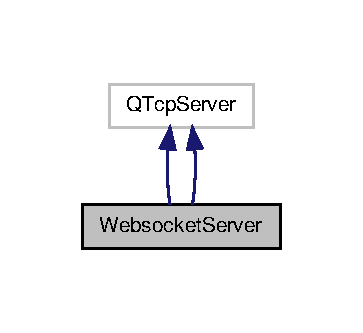
\includegraphics[width=174pt]{class_websocket_server__inherit__graph}
\end{center}
\end{figure}


Collaboration diagram for Websocket\-Server\-:
\nopagebreak
\begin{figure}[H]
\begin{center}
\leavevmode
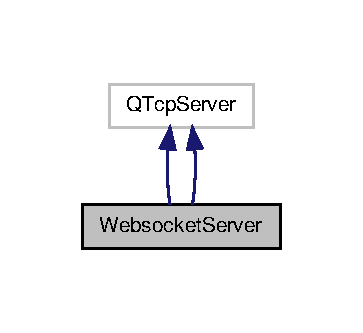
\includegraphics[width=174pt]{class_websocket_server__coll__graph}
\end{center}
\end{figure}
\subsection*{Public Member Functions}
\begin{DoxyCompactItemize}
\item 
\hyperlink{class_websocket_server_a1c00121c9499569f5ab90bf5d71f5e17}{Websocket\-Server} (Q\-Object $\ast$parent=0)
\begin{DoxyCompactList}\small\item\em \hyperlink{class_websocket_server}{Websocket\-Server} websocket server build object. \end{DoxyCompactList}\item 
\hypertarget{class_websocket_server_a0ee0b45831865c20f40a4a1fc8a1e6a1}{\hyperlink{class_websocket_server_a0ee0b45831865c20f40a4a1fc8a1e6a1}{$\sim$\-Websocket\-Server} ()}\label{class_websocket_server_a0ee0b45831865c20f40a4a1fc8a1e6a1}

\begin{DoxyCompactList}\small\item\em \hyperlink{class_websocket_server_a0ee0b45831865c20f40a4a1fc8a1e6a1}{Websocket\-Server\-::$\sim$\-Websocket\-Server} desctruct =$>$ delete pointers. \end{DoxyCompactList}\item 
void \hyperlink{class_websocket_server_ac83322fab8d8ba8d866eae29c61e8cc5}{add\-Client\-Event\-Listener} (\hyperlink{class_i_client_event_listener}{I\-Client\-Event\-Listener} $\ast$client\-Listener)
\begin{DoxyCompactList}\small\item\em \hyperlink{class_websocket_server_ac83322fab8d8ba8d866eae29c61e8cc5}{Websocket\-Server\-::add\-Client\-Event\-Listener} add a client event listener to list. \end{DoxyCompactList}\item 
\hyperlink{class_websocket_server_a1c00121c9499569f5ab90bf5d71f5e17}{Websocket\-Server} (Q\-Object $\ast$parent=0)
\begin{DoxyCompactList}\small\item\em \hyperlink{class_websocket_server}{Websocket\-Server} websocket server build object. \end{DoxyCompactList}\item 
void \hyperlink{class_websocket_server_ac83322fab8d8ba8d866eae29c61e8cc5}{add\-Client\-Event\-Listener} (\hyperlink{class_i_client_event_listener}{I\-Client\-Event\-Listener} $\ast$client\-Listener)
\begin{DoxyCompactList}\small\item\em \hyperlink{class_websocket_server_ac83322fab8d8ba8d866eae29c61e8cc5}{Websocket\-Server\-::add\-Client\-Event\-Listener} add a client event listener to list. \end{DoxyCompactList}\end{DoxyCompactItemize}
\subsection*{Static Public Attributes}
\begin{DoxyCompactItemize}
\item 
static std\-::map$<$ Q\-Tcp\-Socket \\*
$\ast$, \hyperlink{class_client_socket}{Client\-Socket} $>$ \hyperlink{class_websocket_server_acfa614b7fed5046d8cf7ca65baabb275}{socket\-Client\-List}
\begin{DoxyCompactList}\small\item\em socket\-Client\-List socket client list \end{DoxyCompactList}\end{DoxyCompactItemize}


\subsection{Detailed Description}
The \hyperlink{class_websocket_server}{Websocket\-Server} class Websocket server main process class. 

websocketserver.\-h

Websocket server main process class

manage incoming connections manage socket encryption for S\-S\-L socket manage process of incoming data from client socket

\begin{DoxyAuthor}{Author}
Bertrand Martel 
\end{DoxyAuthor}
\begin{DoxyVersion}{Version}
1.\-0 
\begin{DoxyItemize}
\item manage incoming connections 
\item manage socket encryption for S\-S\-L socket 
\item manage process of incoming data from client socket 
\end{DoxyItemize}
\end{DoxyVersion}

\begin{DoxyItemize}
\item manage incoming connections 
\item manage socket encryption for S\-S\-L socket 
\item manage process of incoming data from client socket 
\end{DoxyItemize}

\subsection{Constructor \& Destructor Documentation}
\hypertarget{class_websocket_server_a1c00121c9499569f5ab90bf5d71f5e17}{\index{Websocket\-Server@{Websocket\-Server}!Websocket\-Server@{Websocket\-Server}}
\index{Websocket\-Server@{Websocket\-Server}!WebsocketServer@{Websocket\-Server}}
\subsubsection[{Websocket\-Server}]{\setlength{\rightskip}{0pt plus 5cm}Websocket\-Server\-::\-Websocket\-Server (
\begin{DoxyParamCaption}
\item[{Q\-Object $\ast$}]{parent = {\ttfamily 0}}
\end{DoxyParamCaption}
)}}\label{class_websocket_server_a1c00121c9499569f5ab90bf5d71f5e17}


\hyperlink{class_websocket_server}{Websocket\-Server} websocket server build object. 

\hyperlink{class_websocket_server_a1c00121c9499569f5ab90bf5d71f5e17}{Websocket\-Server\-::\-Websocket\-Server} construct for websocket server init new connection signal and set consumer.


\begin{DoxyParams}{Parameters}
{\em parent} & \\
\hline
\end{DoxyParams}
\hypertarget{class_websocket_server_a1c00121c9499569f5ab90bf5d71f5e17}{\index{Websocket\-Server@{Websocket\-Server}!Websocket\-Server@{Websocket\-Server}}
\index{Websocket\-Server@{Websocket\-Server}!WebsocketServer@{Websocket\-Server}}
\subsubsection[{Websocket\-Server}]{\setlength{\rightskip}{0pt plus 5cm}Websocket\-Server\-::\-Websocket\-Server (
\begin{DoxyParamCaption}
\item[{Q\-Object $\ast$}]{parent = {\ttfamily 0}}
\end{DoxyParamCaption}
)}}\label{class_websocket_server_a1c00121c9499569f5ab90bf5d71f5e17}


\hyperlink{class_websocket_server}{Websocket\-Server} websocket server build object. 


\begin{DoxyParams}{Parameters}
{\em parent} & \\
\hline
\end{DoxyParams}


\subsection{Member Function Documentation}
\hypertarget{class_websocket_server_ac83322fab8d8ba8d866eae29c61e8cc5}{\index{Websocket\-Server@{Websocket\-Server}!add\-Client\-Event\-Listener@{add\-Client\-Event\-Listener}}
\index{add\-Client\-Event\-Listener@{add\-Client\-Event\-Listener}!WebsocketServer@{Websocket\-Server}}
\subsubsection[{add\-Client\-Event\-Listener}]{\setlength{\rightskip}{0pt plus 5cm}void Websocket\-Server\-::add\-Client\-Event\-Listener (
\begin{DoxyParamCaption}
\item[{{\bf I\-Client\-Event\-Listener} $\ast$}]{client\-Listener}
\end{DoxyParamCaption}
)}}\label{class_websocket_server_ac83322fab8d8ba8d866eae29c61e8cc5}


\hyperlink{class_websocket_server_ac83322fab8d8ba8d866eae29c61e8cc5}{Websocket\-Server\-::add\-Client\-Event\-Listener} add a client event listener to list. 


\begin{DoxyParams}{Parameters}
{\em client\-Listener} & client listener \\
\hline
\end{DoxyParams}
\hypertarget{class_websocket_server_ac83322fab8d8ba8d866eae29c61e8cc5}{\index{Websocket\-Server@{Websocket\-Server}!add\-Client\-Event\-Listener@{add\-Client\-Event\-Listener}}
\index{add\-Client\-Event\-Listener@{add\-Client\-Event\-Listener}!WebsocketServer@{Websocket\-Server}}
\subsubsection[{add\-Client\-Event\-Listener}]{\setlength{\rightskip}{0pt plus 5cm}void Websocket\-Server\-::add\-Client\-Event\-Listener (
\begin{DoxyParamCaption}
\item[{{\bf I\-Client\-Event\-Listener} $\ast$}]{client\-Listener}
\end{DoxyParamCaption}
)}}\label{class_websocket_server_ac83322fab8d8ba8d866eae29c61e8cc5}


\hyperlink{class_websocket_server_ac83322fab8d8ba8d866eae29c61e8cc5}{Websocket\-Server\-::add\-Client\-Event\-Listener} add a client event listener to list. 


\begin{DoxyParams}{Parameters}
{\em client\-Listener} & client listener \\
\hline
\end{DoxyParams}


\subsection{Member Data Documentation}
\hypertarget{class_websocket_server_acfa614b7fed5046d8cf7ca65baabb275}{\index{Websocket\-Server@{Websocket\-Server}!socket\-Client\-List@{socket\-Client\-List}}
\index{socket\-Client\-List@{socket\-Client\-List}!WebsocketServer@{Websocket\-Server}}
\subsubsection[{socket\-Client\-List}]{\setlength{\rightskip}{0pt plus 5cm}static std\-::map$<$ Q\-Tcp\-Socket $\ast$, {\bf Client\-Socket} $>$ Websocket\-Server\-::socket\-Client\-List\hspace{0.3cm}{\ttfamily [static]}}}\label{class_websocket_server_acfa614b7fed5046d8cf7ca65baabb275}


socket\-Client\-List socket client list 

\hyperlink{class_websocket_server_acfa614b7fed5046d8cf7ca65baabb275}{Websocket\-Server\-::socket\-Client\-List} static list featuring all socket client connected to server. 

The documentation for this class was generated from the following files\-:\begin{DoxyCompactItemize}
\item 
/home/abathur/\-Bureau/open\-\_\-source/websocketcpp/libwebsocket/protocol/websocket/websocketserver.\-h\item 
/home/abathur/\-Bureau/open\-\_\-source/websocketcpp/libwebsocket/release/protocol/websocket/websocketserver.\-h\item 
/home/abathur/\-Bureau/open\-\_\-source/websocketcpp/libwebsocket/protocol/websocket/websocketserver.\-cpp\end{DoxyCompactItemize}

%--- End generated contents ---

% Index
\newpage
\phantomsection
\addcontentsline{toc}{part}{Index}
\printindex

\end{document}
